%preamble - package inclusion and set up
\documentclass[10pt,oneside,a4paper,english]{paper} %normalt 12pt og twoside
% Select encoding of your inputs
\usepackage[utf8]{inputenc}

% Make latex understand and use the typographic
% rules of the language used in the document.
%\usepackage[danish]{babel}
\usepackage[english]{babel}

% Use the vector font Latin Modern which is going
% to be the default font in latex in the future.
\usepackage{lmodern}

% Choose the font encoding
\usepackage[scaled]{helvet}
\renewcommand\familydefault{\sfdefault} 
\usepackage[T1]{fontenc}

% Use color in tables
\usepackage[table]{xcolor}
\usepackage{pbox}
\usepackage{tabularx}
\usepackage{array}
\usepackage{multirow}

% Load a colour package
\usepackage{xcolor}
\definecolor{aaublue}{RGB}{33,26,82}  %<--define aaublue
\definecolor{white}{RGB}{255,255,255} %<--define white

% ref stuffz
\usepackage{cleveref}

% The standard graphics inclusion package
\usepackage{graphicx}

\makeatletter
  \g@addto@macro\@floatboxreset\centering %<--centering all figures
\makeatother

\usepackage{adjustbox}

% Set up how figure and table captions are displayed

\usepackage{float}
\restylefloat{figure}
\usepackage{caption}
\usepackage{subfigure}
\usepackage[subfigure]{tocloft}
\captionsetup
{
  justification = centering,    %<--centering caption with multiple lines
  font          = footnotesize, %<--set font size to footnotesize
  labelfont     = bf            %<--bold label (e.g., Figure 3.2) font
}
\captionsetup[subfigure]
{
  justification = centering, %<--centering subfigure caption text
  singlelinecheck=false,
  font = footnotesize        %<--font size for subfigures
} 

% Enable row combination in tables
\usepackage{multirow}

% Make space between table lines and text
\renewcommand{\arraystretch}{1.5}

% Enable commands like \st (strike out) and \hl (high light)
\usepackage{soul}

% Make the standard latex tables look so much better
\usepackage{array,booktabs}

% Enable the use of frames around, e.g., theorems
% The framed package is used in the example environment
\usepackage{framed}
\usepackage{colortbl}
\usepackage{longtable}
\usepackage{xcolor}
\usepackage{textcomp}

%-------MATHEMATICS---------------------------------
% Defines new environments such as equation,
% align and split 
\usepackage{amsmath}
\usepackage{relsize}
% Adds new math symbols
\usepackage{amssymb}
% Use theorems in your document
% The ntheorem package is also used for the example environment
% When using thmmarks, amsmath must be an option as well. Otherwise \eqref doesn't work anymore.
\usepackage[framed,amsmath,thmmarks]{ntheorem}
\usepackage{xifthen}%<--enables ifthenelse which is used in macros

\usepackage{siunitx} 
\sisetup{decimalsymbol=period}%<--\num{} will swich commas with periods
\sisetup{detect-weight}
%---------------------------------------------------

%-------PAGE LAYOUT---------------------------------
% Change margins, papersize, etc of the document
\usepackage[
  left=13mm,% left margin on an odd page %tidligere 25mm for baade right og left 25 normalt på alle
  right=13mm,% right margin on an odd page
  top=19mm, %normalt 35
  bottom=43mm, %normalt ikke defineret
  ]{geometry}
  
% Modify how \chapter, \section, etc. look
% The titlesec package is very configureable
\usepackage{titlesec}
\makeatletter
\def\ttl@mkchap@i#1#2#3#4#5#6#7{%
    \ttl@assign\@tempskipa#3\relax\beforetitleunit
    \vspace{\@tempskipa}%<<<<<< REMOVE THE * AFTER \vspace
    \global\@afterindenttrue
    \ifcase#5 \global\@afterindentfalse\fi
    \ttl@assign\@tempskipb#4\relax\aftertitleunit
    \ttl@topmode{\@tempskipb}{%
        \ttl@select{#6}{#1}{#2}{#7}}%
    \ttl@finmarks  % Outside the box!
    \@ifundefined{ttlp@#6}{}{\ttlp@write{#6}}}
\makeatother

\titlespacing{\chapter}{0pt}{0pt}{10pt}
\titlespacing{\section}{0pt}{0pt}{-5pt}
\titlespacing{\subsection}{0pt}{8pt}{-5pt}
\titlespacing{\subsubsection}{0pt}{6pt}{-10pt}

\titleformat*{\section}{\normalfont\Large\bfseries\color{black}}
\titleformat*{\subsection}{\normalfont\large\bfseries\color{black}}
\titleformat*{\subsubsection}{\normalfont\normalsize\bfseries\color{black}}

\usepackage{titlesec, blindtext, color}
%\color{gray75}{gray}{0.75}
\newcommand{\hsp}{\hspace{20pt}}
\titleformat{\chapter}[hang]{\Huge\bfseries}{\thechapter\hsp\textcolor{aaublue}{|}\hsp}{0pt}{\Huge\bfseries}

% Change the headers and footers
\usepackage{fancyhdr}
\setlength{\headheight}{15pt}
\pagestyle{fancy}
\fancyhf{} %delete everything
\renewcommand{\headrulewidth}{0pt} %remove the horizontal line in the header
\fancyhead[RO,LE]{\color{aaublue}\small\nouppercase\leftmark} %even page - chapter title
\fancyhead[LO]{}
\fancyhead[RE]{} 
\fancyhead[CE]{}
\fancyhead[CO]{}
\fancyfoot[RE,LO]{\thepage}
\fancyfoot[LE,RO]{} %page number on all pages
\fancyfoot[CE,CO]{}

% change first page of all chapters header and footer to fancy style
\makeatletter
\let\ps@plain\ps@fancy
\makeatother

% Do not stretch the content of a page. Instead,
% insert white space at the bottom of the page
\raggedbottom

% Enable arithmetics with length. Useful when typesetting the layout.
\usepackage{calc}
%---------------------------------------------------

\usepackage{appendix}

%-------BIBLIOGRAPHY--------------------------------
%setting references (using numbers) and supporting i.a. Chicargo-style:
\usepackage{etex}
\usepackage{etoolbox}
\usepackage{keyval}
\usepackage{ifthen}
\usepackage{url}
\usepackage{csquotes}
\usepackage[backend=biber, url=true, doi=true, style=numeric, sorting=none]{biblatex}
\addbibresource{setup/bibliography.bib}
%---------------------------------------------------

%-------MISC----------------------------------------
%%% Enables the use FiXme refferences. Syntax: \fxnote{...} %%%
\usepackage[footnote, final, english, silent, nomargin]{fixme}		%!!!! DRAFT OR FINAL?!?!?!?!11!! change later!	
%With "final" instead of "draft" an error will ocure for every FiXme under compilation.

%%% allows use of lorem ipsum (generate i.e. pagagraph 1 to 5 with \lipsum[1-5]) %%%
\usepackage{lipsum}

%%% Enables figures with text wrapped tightly around it %%%
\usepackage{wrapfig}

%%% Section debth included in table of contents (1 = down to sections) %%%
\setcounter{tocdepth}{1}

%%% Section debth for numbers (1 = down to sections) %%%
\setcounter{secnumdepth}{2}

\usepackage{tocloft}
\setlength{\cftbeforetoctitleskip}{0 cm}
\renewcommand{\cftpartpresnum}{Del~}
\let\cftoldpartfont\cftpartfont
\renewcommand{\cftpartfont}{\cftoldpartfont\cftpartpresnum}
%---------------------------------------------------

%-------DANSK SPROG---------------------------------

%\addto\captionsdanish{%
%	\renewcommand{\figurename}{figur}%
%	\let\figureautorefname\figurename%
%	\renewcommand{\tablename}{tabel}%
%	\let\tableautorefname\tablename%
%%	\renewcommand{\equationname}{ligning}%
%%	\let\equationautorefname\equationname%
%	\renewcommand{\chaptername}{Kapitel}%
%	\let\chapterautorefname\chaptername%
%	\renewcommand{\partname}{Del}%
%	\let\partautorefname\partname%
%	\renewcommand{\sectionname}{afsnit}%
%	\let\sectionautorefname\sectionname%
%%	\renewcommand{\thesubsection}{underafsnit}%
%%	\let\subsectionautorefname\thesubsection%
%	\renewcommand{\pagename}{side}%
%	\let\pageautorefname\pagename%
%}

%-------HYPERLINKS----------------------------------
% Enable hyperlinks and insert info into the pdf
% file. Hypperref should be loaded as one of the 
% last packages
\usepackage{nameref}
\usepackage{hyperref}
\usepackage{bookmark}
\hypersetup{%
	%pdfpagelabels=true,%
	plainpages=false,%
	pdfauthor={Author(s)},%
	pdftitle={Title},%
	pdfsubject={Subject},%
	bookmarksnumbered=true,%
	colorlinks,%
	citecolor=aaublue,%
	filecolor=aaublue,%
	linkcolor=aaublue,% you should probably change this to black before printing
	urlcolor=aaublue,%
	pdfstartview=FitH%
}

\crefname{appsec}{bilag}{bilag}
%---------------------------------------------------

% remove all indentations
\setlength\parindent{0pt}
\parskip 5mm
\usepackage{verbatim}

\definecolor{Gra}{RGB}{230,230,230}

%creates a nice-looking C#-text
\newcommand{\CC}{C\nolinebreak\hspace{-.05em}\raisebox{.3ex}{\scriptsize\text \#} }

%enables multi column lists
\usepackage{multicol}

%enables code-examples
\usepackage{listings}

\definecolor{coolblue}{RGB}{32,95,128}
\definecolor{mygreen}{rgb}{0,0.6,0}
\definecolor{mygray}{rgb}{0.5,0.5,0.5}
\definecolor{mymauve}{rgb}{0.58,0,0.82}
\usepackage{textcomp}
\definecolor{listinggray}{gray}{0.9}
\definecolor{lbcolor}{rgb}{0.9,0.9,0.9}

%for c code
\lstdefinestyle{cstyle}{
  backgroundcolor=\color{lbcolor},
	tabsize=4,
	rulecolor=,
	language=C,
  basicstyle=\scriptsize,
  upquote=true,
  aboveskip={1.5\baselineskip},
  columns=fixed,
  showstringspaces=false,
  extendedchars=true,
  breaklines=true,
  prebreak = \raisebox{0ex}[0ex][0ex]{\ensuremath{\hookleftarrow}},
  frame=single,
  showtabs=false,
  numbers=left,
  captionpos=b,
  numbersep=5pt,
  numberstyle=\tiny\color{mygray},
  showspaces=false,
  showstringspaces=false,
  identifierstyle=\ttfamily,
  keywordstyle=\color[rgb]{0,0,1},
  commentstyle=\color[rgb]{0.133,0.545,0.133},
  stringstyle=\color[rgb]{0.627,0.126,0.941},
}
%for python code
\lstdefinestyle{pythonstyle}{
    backgroundcolor=\color{lbcolor},
    tabsize=4,
    rulecolor=,
    language=python,
    basicstyle=\scriptsize,
    upquote=true,
    aboveskip={1.5\baselineskip},
    columns=fixed,
    showstringspaces=false,
    extendedchars=true,
    breaklines=true,
    prebreak = \raisebox{0ex}[0ex][0ex]{\ensuremath{\hookleftarrow}},
    frame=single,
    showtabs=false,
    numbers=left,
    captionpos=b,
    numbersep=5pt,
    numberstyle=\tiny\color{mygray},
    showspaces=false,
    showstringspaces=false,
    identifierstyle=\ttfamily,
    keywordstyle=\color[rgb]{0,0,1},
    commentstyle=\color[rgb]{0.133,0.545,0.133},
    stringstyle=\color[rgb]{0.627,0.126,0.941},
}
%for matlab code
\lstdefinestyle{matlabstyle}{
    backgroundcolor=\color{lbcolor},
    tabsize=4,
    rulecolor=,
    language=Matlab,
    basicstyle=\scriptsize,
    upquote=true,
    aboveskip={1.5\baselineskip},
    columns=fixed,
    showstringspaces=false,
    extendedchars=true,
    breaklines=true,
    prebreak = \raisebox{0ex}[0ex][0ex]{\ensuremath{\hookleftarrow}},
    frame=single,
    showtabs=false,
    numbers=left,
    captionpos=b,
    numbersep=5pt,
    numberstyle=\tiny\color{mygray},
    showspaces=false,
    showstringspaces=false,
    identifierstyle=\ttfamily,
    keywordstyle=\color[rgb]{0,0,1},
    commentstyle=\color[rgb]{0.133,0.545,0.133},
    stringstyle=\color[rgb]{0.627,0.126,0.941},   
}

%for java code
\lstdefinestyle{javastyle}{
	backgroundcolor=\color{lbcolor},
	tabsize=4,
	rulecolor=,
	language=Java,
	basicstyle=\scriptsize,
	upquote=true,
	aboveskip={1.5\baselineskip},
	columns=fixed,
	showstringspaces=false,
	extendedchars=true,
	breaklines=true,
	prebreak = \raisebox{0ex}[0ex][0ex]{\ensuremath{\hookleftarrow}},
	frame=single,
	showtabs=false,
	numbers=left,
	captionpos=b,
	numbersep=5pt,
	numberstyle=\tiny\color{mygray},
	showspaces=false,
	showstringspaces=false,
	identifierstyle=\ttfamily,
	keywordstyle=\color[rgb]{0,0,1},
	commentstyle=\color[rgb]{0.133,0.545,0.133},
	stringstyle=\color[rgb]{0.627,0.126,0.941},
}

%for inline c, syntax: \cline{ codeHere(); }
\lstdefinestyle{cinline}{
    style=cstyle,
    basicstyle=\small,
}
\newcommand\inlinec[1]{ \lstinline[style=cinline]{#1} }

%for inline python, syntax: \pythonline{ codeHere(); }
\lstdefinestyle{pythoninline}{
    style=pythonstyle,
    basicstyle=\small,
}
\newcommand\inlinepython[1]{ \lstinline[style=pythoninline]{#1} }

%for inline matlab, syntax: \matlabline{ codeHere(); }
\lstdefinestyle{matlabinline}{
    style=matlabstyle,
    basicstyle=\small,
}
\newcommand\inlinematlab[1]{ \lstinline[style=matlabinline]{#1} }

\usepackage{enumitem}
%\usepackage[citestyle=authoryear,natbib=true]{biblatex}

% Figures - TIKZ
\usepackage{tikz}
\usepackage[americanresistors,americaninductors,americancurrents, americanvoltages]{circuitikz}

% Wall of text logo
\newcommand{\walloftextalert}[0]{\includegraphics[width=\textwidth]{walloftext.png}}

\usepackage{pdfpages}
\usepackage{lastpage}
\usepackage{epstopdf}

\setlength{\headheight}{21pt}

\hfuzz=\maxdimen
\tolerance = 10000
\hbadness  = 10000

\usepackage{siunitx}
\graphicspath{{./figures/}}

%macros - please read this file
%Macro for 'where'-enviroment was improved by Andrea and Niels :-)

%-----------UNITS-------------------------------------------
\newcommand{\unit}[1]{&& \left[\si{#1}\right]}
%
%\newcommand{\unit}[1]{[\si{#1}]}            %<<| Use these if you want equations to be
%\newcommand{\eq}[2]{&&\si{#1} &= \si{#2}&&} %<<| centered.. .. will appear scrambled
%                                            %  | from one equation to the next though..
%                                            %  | and does not work with long equations.. :/
%
%-----------------------------------------------------------

%-----------WHERE ENVIRONMENT-------------------------------
\newenvironment{where}{\leavevmode{\parindent=1em\indent} Where:\\}{}
\newcommand{\va}[3]
{
  \begin{tabular}{p{20pt} p{40pt} p{290pt} l}
    & { $#1$ } & { #2 } & \ifthenelse{\isempty{ #3 }}  {}  {[{\si{#3}}]} \\
  \end{tabular}\\
}
%-----------------------------------------------------------

%-----------TikZ SETTINGS-----------------------------------
\tikzset{
  block/.style    = {draw, thick, rectangle,
                     minimum height = 2.1em,
                     minimum width = 1.7em},
  sum/.style      = {draw, circle, inner sep=3pt} %<--Adder
}
%-----------------------------------------------------------


%-----------Fanzy reference SETTINGS------------------------
%Figure references:
\newcommand{\figref}[1]{figure \ref{#1}}

%Figure references after full stop/period:
\newcommand{\Figref}[1]{Figure \ref{#1}}

%Table references:
\newcommand{\tabref}[1]{table \ref{#1}}

%Table references after full stop/period:
\newcommand{\Tabref}[1]{Table \ref{#1}}

%Section references:
\newcommand{\secref}[1]{section \ref{#1} on page \pageref{#1}}

%Section references:
\newcommand{\Secref}[1]{Section \ref{#1} on page \pageref{#1}}

%Appendix references:
\newcommand{\appref}[1]{appendix \ref{#1} on page \pageref{#1}}

%Appendix references:
\newcommand{\Appref}[1]{Appendix \ref{#1} on page \pageref{#1}}

%chapter references: 
\newcommand{\chapref}[1]{chapter \ref{#1} on page \pageref{#1}}

%chapter references: 
\newcommand{\Chapref}[1]{Chapter \ref{#1} on page \pageref{#1}}

%Units:
%\newcommand{\unit}[1]{&& \left[\si{#1}\right]}

%Text:
\newcommand{\tx}[1]{\text{#1}}

%Equation references:
%1 equation:
\renewcommand{\eqref}[1]{equation (\ref{#1})}

%-----------------------------------------------------------





\begin{document}       % TIP: If you are using TeXstudio you can open
%\tableofcontents      %      the file by Ctrl+LeftClick on setup/macros.tex
%\pagebreak             %      If the file doesn't exist, you will be asked
					   %      weather or not you want to create it.
%\begin{center}
%	\vspace{5cm}
%	\Huge{Worksheets}
%\end{center}
%\clearpage

%||||||||||||||||||||||||||||||||||||||||||||||||||||||||||||||||
%|||||||                 Example Inputs                  ||||||||
%||||||||||||||||||||||||||||||||||||||||||||||||||||||||||||||||
%|||||||                                                 ||||||||
%			 \chapter{Figure Sample}

\begin{figure}[H]                                         %   File-type can be specified
  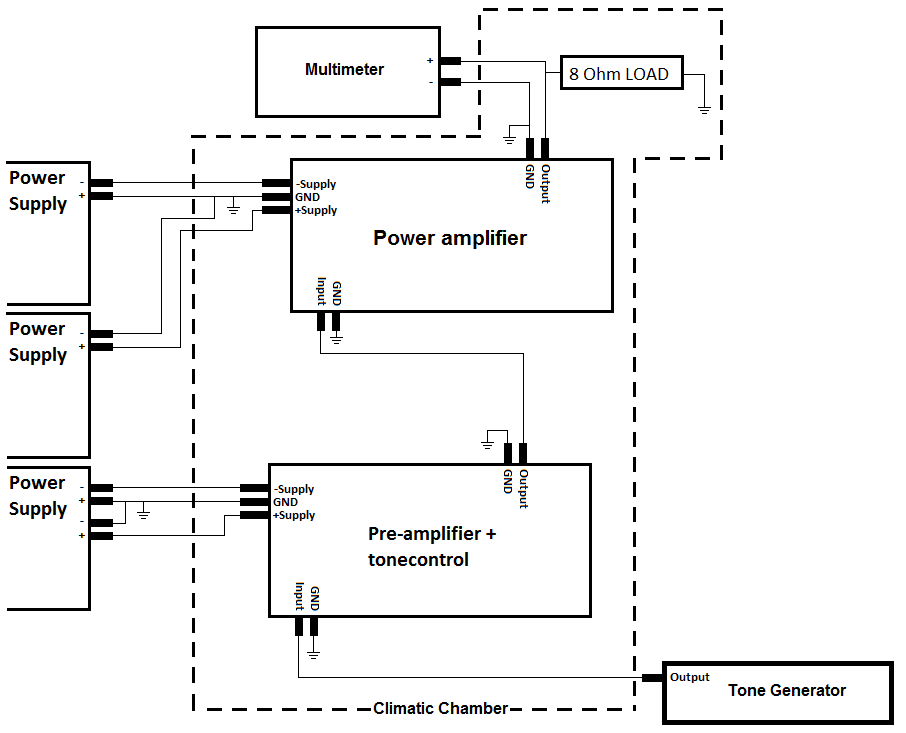
\includegraphics[width=.4\textwidth]{figures/filename}  %<--but is not needed.
  \caption{This image is clearly too small, remember to scale appropriately \fxnote{Remember source}}
  \label{fig:FigureLABEL}  %<--give the figure a label, so you can reference!
\end{figure}               %   For the label to work it must be under the caption.

% Fxnotes will not compile properly inside the figure, only in the caption.
% When \fxnote{} is used in caption, it does not show in a footnote as it normally 
% would, it does however appear in list of corrections.

\autoref{fig:FigureLABEL} $\leftarrow$ use autoref, unless you are referring to multiple pictures, then do like this: \autoref{fig:HbridgeClokwise4Q} and \ref{fig:HbridgeCounterClokwise4Q}.

%Do NOT use \vspace{length}, \hspace{length} or \noindent etc. unless exceedingly necessary - LaTeX is a markup language, let it do its job.
\vspace{.5cm}
\noindent
%
%--------- BIBLIOGRAPHY REF EKSAMPLE -----------------------------------
This reference only represents this line since it is before the punctuation mark\cite{YDing}. This next reference however represents the entire section. That is, all of the preceding sentences in the entire section. This is due to the fact that it is now after the punctuation mark in the end of the section (this is not used in the middle of a section!).\cite{YDing}

%>>PLEASE ALSO READ THE NOTE IN bibliography/bibliography.bib<<

Here is a way to make two images appear on the side of each other. Also, if you modified an image, this is how you properly refer to its original source:

\begin{figure}[H]
    \subcaptionbox  %<--use captionbox instead if no global caption is needed
    {               %                                \%-%-%-%-%-%-%\
      Clockwise 4Q operation.\newline                              %\
      \emph{Edited from image by Biezl.\cite{Biezl}}                %\
      \label{fig:HbridgeClokwise4Q}                                  %\
    }                                                                 %\
    {                                                                  %\
      \includegraphics[width=.46\textwidth]{HbridgeClockwise4Q}         %\
    }                                                                    %\
    \hspace{5pt}                                                          %\
    \subcaptionbox  %<-----------------------------------------------------%\
    {                                                                       %\
      Counterclockwise 4Q operation.\newline                                 %\
      \emph{Edited from image by Biezl.\cite{Biezl}}                          %\
      \label{fig:HbridgeCounterClokwise4Q}                                     %\
    }                                                                           %\
    {                                                                            %\
      \includegraphics[width=.46\textwidth]{HbridgeCounterClockwise4Q}            %|
    }                                                                             %|
    \caption{The 4 quadrant H-bridge configuration shown in both directions.}%<-%-/
    \label{fig:Hbridges}
\end{figure}

As seen \autoref{fig:HbridgeCounterClokwise4Q} can be referred to on its own, or you can use \autoref{fig:Hbridges} to refer to both \autoref{fig:HbridgeClokwise4Q} and \autoref{fig:HbridgeCounterClokwise4Q}.

If the figures are not directly related you might not want to use \textbf{(a)} and \textbf{(b)}, but instead give each figure their own label, here is an example:

\begin{figure}[H]
    \captionbox
    {
      Clockwise 4Q operation.\newline
      \emph{Edited from image by Biezl.\cite{Biezl}}
      \label{fig:HbridgeClokwise4Q2}
    }
    {
      \includegraphics[width=.46\textwidth]{HbridgeClockwise4Q}
    }
    \hspace{5pt}
    \captionbox
    {
      Counterclockwise 4Q operation.\newline
      \emph{Edited from image by Biezl.\cite{Biezl}}
      \label{fig:HbridgeCounterClokwise4Q2}
    }
    {
      \includegraphics[width=.46\textwidth]{HbridgeCounterClockwise4Q}
    }
\end{figure}

In this case \autoref{fig:HbridgeClokwise4Q2} can be referred to without involving \autoref{fig:HbridgeCounterClokwise4Q2}.

\pagebreak			 %|||||||
%			 \section{Table Sample} %to view this sample properly in the code, the screen must be
                       %wide enough, or you have to disable word-wrap in your editor.
\begin{table}[H]
\begin{tabular}{|l|p{5cm}|l|l|l|}
  \hline %-----------------------------------------------------------------------------------
  \textbf{No.} &\textbf{Description} &\textbf{Min} &\textbf{Max} &\textbf{Requirements}    \\
  \hline %-----------------------------------------------------------------------------------
  1            & Some Text           & Some Text   & Some Text   & Some Text               \\
               &                     &             &             & Some More Text          \\
               &                     &             &             & Text Text               \\
               &                     &             &             & Text Text Text          \\
  \hline %-----------------------------------------------------------------------------------
  2            & Some Text           & Some Text   & Some Text   & Some Text               \\
  \hline %-----------------------------------------------------------------------------------
  3            & By specifying the
                 width of a column
                 (|p\{5cm\}|) the
                 cells in that column
                 will not exceed the
                 specified width but         %Extra whitespace is used only for clarity
                 instead expand              %and will not affect the compiled output.
                 downward.
                                     & Some Text           & Some Text   & Some Text       \\
  \hline %-----------------------------------------------------------------------------------
  4            & Some Text           & Some Text   & Some Text   & Some Text               \\
  \hline %-----------------------------------------------------------------------------------
  \multicolumn{2}{|l|}{Some Text}    & \multicolumn{3}{l|}{Some Text}                      \\
  \hline %-----------------------------------------------------------------------------------
  \multicolumn{2}{|l|}{Text Text}    & \multicolumn{3}{l|}{Text = Text}                    \\
  \multicolumn{2}{|l|}{}             & \multicolumn{3}{l|}{Text = Text}                    \\
  \multicolumn{2}{|l|}{}             & \multicolumn{3}{l|}{Text = Text}                    \\
  \multicolumn{2}{|l|}{}             & \multicolumn{3}{l|}{Text = Text}                    \\
  \multicolumn{2}{|l|}{}             & \multicolumn{3}{l|}{Text = Text}                    \\
  \hline %-----------------------------------------------------------------------------------
  \multicolumn{2}{|l|}{Some Text}    & \multicolumn{3}{l|}{Teeeexxtt}                      \\
  \multicolumn{2}{|l|}{}             & \multicolumn{3}{l|}{\LaTeX}                         \\
  \hline %-----------------------------------------------------------------------------------
\end{tabular}
\caption{This Is a Table\label{table:TableLABEL}}
\end{table}

\autoref{table:TableLABEL} $\leftarrow$ use autoref, unless you are referring to multiple tables, then do like this: \autoref{table:TableLABEL} and \ref{table:TableLABEL}.

\pagebreak 		     %|||||||
%			 \section{Equation Sample} %<--In American English all Important Words in
                          %   Headlines are with Big Letters

% \unit is a macro. It uses SI units and aligns all the units neatly :)

\textbf{A normal equation:}
\begin{flalign}
  J_m \cdot \dot{\omega}_m(t) &= \tau_m(t) - B_m \cdot \omega_m(t) - r_m \cdot f_c(t)& \unit{N \cdot m}
  \label{eq:MotorGearNewtonSecLaw}
\end{flalign}
%
\begin{where}
  \va{ J_m               }{is the motor's inertia}                     {kg \cdot m^2}
  \va{ \omega_m(t)       }{is the angular velocity of the motor}       {rad \cdot s^{-1}}
  \va{ \dot{\omega}_m(t) }{is the angular acceleration of the motor}   {rad \cdot s^{-2}}
  \va{ \tau_m(t)         }{is the torque delivered by the motor}       {N \cdot m}
  \va{ B_m               }{is the motor's friction coefficient}        {N \cdot m \cdot s \cdot rad^{-1}}
  \va{ r_m               }{is the radius of the gear, $G_m$}           {m}
  \va{ f_c(t)            }{is the contact force between the two gears} {N}
\end{where}

\textbf{If you need to write something with numbers:} %<--Do not use \textbf{} as headlines, it is bad practice
                                                      %   use instead \chapter{}, \section{}, \subcaption{}, \subsubsection{}
                                                      %   in that order - never a \subsubsection{} directly under a \section{}
\begin{flalign}
  B      &= \num{2,2}\cdot 10^{-6}  \ \si{N\cdot m \cdot rad^{-1} \cdot s}& \label{eq:eq2} \\ %<-- if you want two equations to
  \tau_c &= \num{0.0016}            \ \si{N\cdot m}                       & \label{eq:eq3}    %    allign in one envirenment,
\end{flalign}                                                                              %    remember \\
%using \num{} ensures the same use of decimal point throughout the repport
%should you want to change it, the option is set in the preamble, just change 'period' to 'comma':
%\sisetup{decimalsymbol=period}

\autoref{eq:MotorGearNewtonSecLaw} $\leftarrow$ use autoref, unless you are referring to multiple equations, then do like this: \autoref{eq:eq2} and \ref{eq:eq3}.

\pagebreak		 %|||||||
%			 \section{TikZ Sample}

\textbf{TikZ is only for very patient people, I can recommend Inkscape with textext plugin: \url{https://pav.iki.fi/software/textext/}, difficult to install easy to use, and, if used carefully, nice results.}

%heavily commented example
\input{chapters/tikz/TikZblockDiagramSample.tex}

%way to keep the drawing code in a seperate file
\begin{figure}[H]
	\input{chapters/tikz/smallBlockDiagram.tikz}
	\centering
	\caption{Block diagram}
\end{figure}

%TikZ can also be used for circuits
\input{chapters/tikz/TikZcircuitSample.tex}


\pagebreak            %|||||||
%			 \section{Code Sample}

\begin{lstlisting}[ style=cstyle,
                    caption={C Code}, 
                    label=lst:cExample ]
#include "functions.h"

// Constant matrices
const float L[3] = { -11.0, -12.0, -13.0 };
const float B1[4] = { 0.0, -0.2396, 0.0, 0.2396 };
const float B2[4] = { 0.2396, 0.0, -0.2396, 0.0 };
const float B3[4] = { 0.0377, -0.0377, 0.0377, -0.0377 };
\end{lstlisting}

In \autoref{lst:cExample} is some C-code, and here is some in-line C-code: \inlinec{xTaskCreate();}.

\begin{lstlisting}[ style=pythonstyle,
                    caption={Python Code}, 
                    label=lst:pythonExample ]
# This parses the packets to identify messages and decodes them for the logs
class packetParser():
    def __init__(self,accelfile,gpsfile,measstate,fulllog,plog):
        self.GPS = {0: 'Latitude',
                    1: 'Longtitude',
                    2: 'Velocity'}
        self.IMU = {0: 'AccelerationX',
                    1: 'AccelerationY',
                    2: 'AccelerationZ',
                    3: 'GyroscopeX',
                    4: 'GyroscopeY',
                    5: 'GyroscopeZ',
                    6: 'MagnetometerX',
                    7: 'MagnetometerY',
                    8: 'MagnetometerZ',
                    9: 'Temperature'}
        self.MsgID = {0: self.GPS, 1: self.IMU}
        self.DevID = {0: 'GPS', 1: 'IMU'}
        self.accelburst = [0,0,0,0,0,0,0]
        self.accellog = accelfile
        self.fulllog = fulllog
\end{lstlisting}

In \autoref{lst:pythonExample} is some Python-code, and here is some in-line Python-code:\\ \inlinepython{self.plog.write(str(msgnr))}

\begin{lstlisting}[ style=matlabstyle,
                    caption={Matlab Code}, 
                    label=lst:matlabExample ]
  close all
  clear
  clc
  
  % Parameters
  mx=200;     % [kg] mass + added mass in xb direction
  my=250;     % [kg] mass + added mass in yb direction
  Iz=700;     % [kgm2]
  
  dx=70;      % [kg/s] 
  dy=100;     % [kg/s]
  dyaw=50;    % [kgm2/s]
\end{lstlisting}

In \autoref{lst:cExample}, \ref{lst:pythonExample} and \ref{lst:matlabExample} is some code, and here is some in-line matlab: \inlinematlab{randn(50)}            %|||||||
%|||||||                                                 ||||||||
%||||||||||||||||||||||||||||||||||||||||||||||||||||||||||||||||
%||||||||||||||||||||||||||||||||||||||||||||||||||||||||||||||||


%%% Prereport %%%
		\setlength\cftaftertoctitleskip{2pt}
		\setlength\cftafterloftitleskip{6pt}
		\setlength\cftafterlottitleskip{6pt}
%\selectlanguage{danish}
%\title{Testing the performance of linear regressors using inertial information combined with sEMG to minimize the limb position effect in proportional and simultaneous control of lower arm prosthetics.}

%%% Frontmatter Settings %%%
		\pagestyle{empty} %disable headers and footers
		\pagenumbering{roman} %use roman page numbering in the frontmatter I II...
%		\fancyfoot[RE,LO]{17gr7404} %page number on all pages
%		\fancyfoot[LE,RO]{\thepage}
%		\fancyhead[LE,LO,RE,RO]{}

%%% Introductory Formalities %%%
%\includepdf[pages={1}]{formalities/frontpage.pdf}
%			\clearpage
\thispagestyle{empty}

\begin{figure}[H]
	\raggedleft
	
\includegraphics[width=0.2\textwidth]{figures/aaulogo-en.png}
\end{figure} 

\vspace{5 cm}

\begin{center}
	\begin{Huge}
		\textbf{Examining if Confidence Score Feedback During User Training Can Improve Users’ Ability in Controlling Upper Limb Prosthetics}\\
		\vspace{5 mm}
		2nd semester Masters, Biomedical Engineering \& Infomatics - Spring $2018$\\
		\vspace{3 mm}
	\end{Huge}
	{\Large Project group: $18$gr$8408$} \\
	\vspace{1cm}
	\large{Simon Bruun, Oliver Thomsen Damsgaard, Martin Alexander Garenfeld, Christian Korfitz Mortensen}
\end{center}
\vspace*{\fill}

\begin{center}
	\line(1,0){400}
\end{center}

%\newpage
%
%\large{\textbf{Project period:}\\
%P7, Autumn 2017\\
%01/08/2017 - 20/12/2017\\
%
%\textbf{Project group:}\\
%17gr7404\\} %\fxnote{Input group number}
%
%
%\begin{center}
%	\Large{\textbf{Collaborators:}\\
%		\vspace{1.5cm}
%	\rule{10cm}{1pt}\\
%	Irene Uriarte \\
%	
%	\rule{10cm}{1pt}\\
%	Martin Alexander Garenfeld \\
%	
%	\rule{10cm}{1pt}\\
%	Oliver Thomsen Damsgaard \\
%	
%	\rule{10cm}{1pt}\\
%	Simon Bruun \\}
%\end{center}
%
%
%
%\large{\textbf{Supervisors:}\\
%Strahinja Dosen \\
%Jakob Lund Dideriksen \\
%Lotte N.S. Andreasen Struijk} \\
%\\
\newpage
			% <--- the frontpage
%			\pagestyle{fancy}
%%{\small
\strut\vfill % push the content to the bottom of the page
\noindent Copyright \copyright{} Aalborg University 2015\par
\vspace{0.2cm}

\noindent This report is compiled in \LaTeX, originally developed by Leslie Lamport, based on Donald Knuth's \TeX. The main text is written in \emph{Latin Modern} pt 12, designed by Bogusław Jackowski and Janusz M. Nowacki. 
%The document is compiled via the website \url{www.overleaf.com}, an online collaborative based \LaTeX-editor with instant preview, which enables multiple persons to edit the document simultaneously.
Flowcharts and diagrams are made using Microsoft Visio. 
\clearpage
%			%\begin{document} 
\thispagestyle{empty}
\begin{titlepage}
\begin{nopagebreak}
{\samepage 

\begin{tabular}{r}
\parbox{\textwidth}{  \raisebox{-15mm}{
\includegraphics[height=3cm]{figures/aaulogo-en.png}}
\hfill \hspace{2cm} \parbox{8cm}{\begin{tabular}{l} %4.90
{\small \textbf{\textcolor{aaublue}{{7\textsuperscript{th} Semester, Masters Project}}}}\\
{\small \textbf{\textcolor{aaublue}{School of Medicine and Health}}}\\
%{\small \textbf{\textcolor{aaublue}{Communication Technologies}}}\\ 
{\small \textbf{\textcolor{aaublue}{Biomedical Engineering and Informatics}}}\\
{\small \textcolor{aaublue}{Fredrik Bajers Vej 7A}} \\
{\small \textcolor{aaublue}{9220 Aalborg}} \\
%{\small \textcolor{aaublue}{\emph{http://www.sict.aau.dk/electronics-and-it}}}
\end{tabular}}}
\end{tabular}

\begin{tabular}{cc}
\parbox{7cm}{

\textbf{The effect of limb position on myoelectric prosthetic control using linear regression}
\\
\textbf{Theme: Biomedical signals and information}

\small{
\\
}


\parbox{8cm}{


\textbf{Project period:}\\
P7, Autumn 2017\\
01/08/2017 - 20/12/2017\\
   
\textbf{Project group:}\\
17gr7404\\ %\fxnote{Input group number}
  
\textbf{Collaborators:}\\
\rule{5cm}{1pt}\\
Irene Uriarte \\
\rule{5cm}{1pt}\\
Martin Alexander Garenfeld \\
\rule{5cm}{1pt}\\
Oliver Thomsen Damsgaard \\
\rule{5cm}{1pt}\\
Simon Bruun \\

\textbf{Supervisors:}\\
Strahinja Dosen \\
Jakob Lund Dideriksen \\
Lotte N.S. Andreasen Struijk \\
}\\


\textbf{Pages:} 0\\
\textbf{Appendixes:} b \\
%\textbf{Ekstra:} For projektkode: Se forord\\ %eks. en CD eller USB
\textbf{Completed:} 19/12/2017\\

\vfill } &
\parbox{7cm}{
  \vspace{.15cm}
  \hfill
  \begin{tabular}{l}
  {\textbf{Abstract}}\bigskip \\
  \fbox{
    \parbox{6.5cm}{\bigskip
     {\vfill{\small \lipsum[15]
%write real thing
     \bigskip}}
     }}
   \end{tabular}}
\end{tabular}} %\vspace{1cm}


\centering
\textit{Publication of this report's contents, including source references, may only happen in agreement with the authors.}\\
%\textit{Offentliggørelse af rapportens indhold, med kildeangivelse, må kun ske efter aftale med forfatterne.}\\


\end{nopagebreak}
\end{titlepage}
%\end{document} 			 % <--- the titlesheet - contains the synopsis!!
%%%% Preface %%%
%			\cleardoublepage
%			%abstract

%\section{Abstract}					%prolly not needed

%clever abstract below
The user rejection rate of myoelectric prosthetics is currently high, due to slow and inaccurate control. Previous studies have shown user training to be an important part of overcoming the challenge of making transradial upper limb prosthetics more accurate, as the control systems depend on the user generating the same distinguishable muscle patterns when using the prosthesis. Different methods have been sought when adapting users to perform specific distinguishable movements. This study aimed to investigate whether confidence score feedback from a LDA classifier during user training could improve user performance in a Fitts' Law test compared to a control group who only received label feedback. %The study will be designed to examine prosthetic control in lower arm prosthetics.
16 able-bodied subjects were recruited for the study; 8 subjects randomly assigned to each group. Each subject went through a three session experiment; one session per day over three consecutive days. During each session the subject received a 16 minutes user training and went subsequently through a Fitts' Law test to evaluate the performance.
%, where they were instructed to perform six different hand movements in three intensities during data acquisition. This was then used to build a LDA based classifier the subjects were to use during the training, teaching them to perform specific movements at different intensities. Afterwards they were subjected to a Fitts' Law based test in a GUI to examine their ability to perform the trained movements. These steps were repeated for three sessions over three consecutive days.
A significant improvement in cluster dispersion of EMG signals of separate movement was found in the control group, where the third session resulted in more dense clusters both when compared to the first session of the control group and third session of the test group. The results from the Fitts' Law test showed no significant difference between the two groups and no improvement over the three sessions for either of the groups. Overall, three sessions of user training with confidence score feedback showed to be an insufficient training period to observe a significant improvement within and between subject groups.

\textit{\textbf{Keywords: surface electromyography, lower arm prosthetics, linear discriminant analysis, user training, confidence scores}}			 % <--- this is the abstract!!
%%\clearpage
%			\chapter*{Preface}

\lipsum[9]

\pagebreak				% <--- the preface
%
%			\pdfbookmark[0]{Table of Contents}{label: tableOfCentents}
%			\tableofcontents
%%			\cleardoublepage


%%% Mainmatter Settings %%%
\pagenumbering{arabic} %use arabic page numbering in the mainmatter
\fancyhf{}
\fancyfoot[C]{\thepage} %\text{ of} \pageref{LastPage}			% ADD LABLE{LASTPAGE} TO LAST PAGE !!
\fancyfoot[RE,LO]{18gr8408}																								   %
\fancyhead[RE,LO]{}																												%% } consider fancyfoots
\fancyhead[RE,LO]{\color{aaublue}\small\nouppercase\leftmark} %even page - chapter title %
\pagestyle{fancy}


%---------------------------INPUTS-------------------------------

%%statusseminar text

\chapter*{Using estimation uncertainty to improve prosthesis control}

\textbf{Group 8408. Simon Bruun, Oliver Damsgaard, Martin Garenfeld, Christian Mortensen}

\section*{Introduction}

Electromyography (EMG) is the recording and utilization of muscle generated electric potentials, widely used in control of functional prosthetics. The electric potentials recorded from the muscles are action potentials generated by the activation of a muscle contraction. The contraction force a muscle produce is related to the intensity of an EMG recording. The recorded EMG signals are processed through several steps of amplification, filtering and feature extraction before they are used as input in the control for a myoelectric prosthesis. \cite{Cram2012, Fougner2012}

Myoelectric prosthetics are becoming increasingly advanced, however they still suffer commercial success due to lack of usability outside clinical environments. \cite{Hwang2017, Jiang2012, Scheme2010} Thus, many users reject the use of the prosthetics. 
In recent years development in myoelectric prosthetics have been greatly focused on refining classification accuracy, while other research areas have been more or less neglected \cite{Jiang2012}. However, there still exist a challenge for the users to be able to consistently produce distinguishable muscle patterns, and the better these muscle patterns the better the system will function. \cite{Powell2014} Far fewer studies have been made on user training when compared to studies on system training, though the significance of user training is not doubted \cite{Fang2017}. Powell et. al conclude that in order for amputees to understand the significance of producing consistent and distinguishable muscle patterns, the need for user training is important \cite{Powell2013}.

Fang et. al \cite{Fang2017} evaluated the progress of the human learning ability in a pattern recognition based control scheme when providing classifier-feedback during user training. Here, a clustering-feedback method based on Principal Component Analysis (PCA) was used to provide users with real-time visual feedback, to guide users to correctly perform movements based on the recorded EMG signals. The visual feedback consisted of a map with dots representing centroids of classes. Through control based on an Linear Discriminant Analysis (LDA) classifier, users could match the control input to these centroids to best perform a movement to be classified correctly. The study showed great improvements for user training, and an ability to quicken the learning for amputees who are unfamiliar with EMG controlled prosthetic use. \cite{Fang2017}
Powell et. al \cite{Powell2014} demonstrated, by using an LDA classifier, an increase in movement completion percentage from 70.8\% to 99.0\%, a decrease in movement completion time from 1.47 to 1.13, as well as a significant improvement in classifier accuracy from 77.5\% to 94.4\%, for users undergoing user training for a two week period. This study provided feedback through a virtual animated prosthesis.
Pan et. al \cite{Pan2017} provided a visual feedback of an arrow to be moved on a 2D plane. Pan et. al also tested the effect of stimulating the subjects’ brain with transcranial direct current stimulation (tDCS). The study concluded that tDCS together with user training provided significantly better results than user training alone. \cite{Pan2017}

The general challenge of user training is for the user to be able to consistently produce distinguishable muscle patterns. \cite{Powell2014} Therefore further research in user training could provide a vital leap towards more precise classification using current methods, as well as a faster user adaptation of myoelectric controlled prosthetics, but an effective way to properly provide feedback to the user have yet to be developed. 
Further studies should for now concentrate on developing different feedback methods which should later be compared to determine an ideal method. 
This study will seek to develop a new method of feedback during user training, by providing the users with the estimation uncertainty of the classification. To the authors knowledge, user feedback has not been provided with this method before.

\section*{Methods}

%This study will utilize classification and probability estimation based on EMG recordings to evaluate and compute uncertainty estimations for classifying four different hand gestures. The goal is to develop a system that use the classification uncertainties to improve user training.

%The study will consist of steps of data acquisition, user training and an online test. The user will undergo user training followed by a targets reaching Fitts' Law test. The study will have a test and control group, where the control group will be trained without visual feedback during user training. Post hoc statistic comparisons will be made between online tests and maybe some other things we have not entirely decided upon yet.

\textbf{Data acquisition} will be done with a Myo armband (MYB) from Thalmic Labs. The MYB contains eight surface EMG electrodes, which has a sampling rate of 200 Hz.
For \textbf{feature extraction} four features will be extracted from the acquired data; slope-sign changes (SSC), waveform length (WL), zero crossings (ZC) and mean absolute value (MAV). The features will be extracted from a window of 200 ms (40 samples) with a 50\% overlap.
For \textbf{classification} LDA will be used. LDA is a supervised classification method used to separate classes of data by linear decision boundaries. Classification methods attempt to classify similar patterns in EMG signals, between previously acquired data and new data \cite{Mendez2017}. In LDA each decision boundary is a hyperplane from which the minimum distance from the classes it separates is maximized, and the distance from the means of the classes are maximized. A decision boundary is defined as a linear combination of the feature values.
Evaluating the certainty that a feature value belongs to a given class can be done by computing the posterior probability of each class. The posterior probability is a value between 0 and 1. The posterior probability is given as the product of the class conditional probability and the prior probability divided by a normalization term that guaranties that the posterior probabilities for all classes sums to one. The class conditional probability is the probability of obtaining a feature value when selecting samples randomly from a class. The prior probability is the likelihood that a sample from a class appears when compared to the other classes before it actually has appeared.

The effect of user training with and without providing uncertainty estimations during the user training, will be tested through a target reaching test. The test will executed in a virtual environment. During the test the user must reach targets of varying size and distance to each other. The test evaluates users speed to reach targets, accuracy, overshoot and overall completion rate \cite{Scheme2013}. 
Lastly a \textbf{statistical} analysis will be used to compare results of the target reaching test between users training with and without provided estimated uncertainty during user training.


\section*{Study protocol}

\textbf{Research question/hypothesis}

Using uncertainty estimation as visual feedback during user training will improve the users performance in a linear discriminant controlled target reaching test based on electromyography recordings.

\textbf{Ethical considerations}  

The investigators do not foresee any obstacles of ethical nature during the proceedings of this experiment. No test subjects will be exposed to any physical interventions besides being asked to wear the Myo armband. No part of this experiment should put the subject in danger. 

\textbf{Session time}

The experiment consist of one session divided into two sub-sessions with an estimated total duration of 2-3 hours.

\textbf{Inclusion criteria}

The subject needs to be:
\begin{itemize}
	\item able bodied.
	\item between 18 and 35 years of age.
	\item able to understand and speak Danish and/or English.
	\item assessed by the investigators to understand and perform the instructions given during the experiment. 
\end{itemize}


\textbf{Exclusion criteria}

The subject must not have:
\begin{itemize}
	\item diseases that, assessed by the investigators, might influence subject performance.
\end{itemize}


\textbf{Experiment procedure}

The experiment is divided into two sessions: 1) training data acquisition, user training and performance test and 2) new training data acquisition and performance test. During the training data acquisition EMG data will be recorded from the subject with an EMG-electrode armband (Myoband from Thalmic Labs) when performing four different wrist movements (flexion, extension, radial deviation and ulnar deviation). The data is subsequently used to fit a classification model used in the myoelectric control scheme for the following user training and performance test. Before the performance test the user is given a training period to get familiar with wrist movements used in the performance test. During the performance test the subject will perform a target-reaching task in a cartesian coordinate system of reaching a number of targets using wrist movements, where each axis represent a one of four wrist movements. The aim for the subject is to reach as many targets as quickly as possible. The subject will perform the target-reaching task twice - one in each session. The subjects are divided into two groups: a test group and a control group. As the study is single-blinded the subject will not be informed which group he/she belongs to.

\begin{figure}[H]                                         
	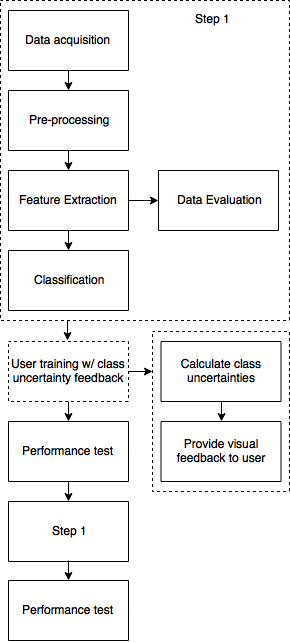
\includegraphics[width=.4\textwidth]{figures/sStatusSeminar/systemPepeLineTG}  
	\caption{System pipeline for the test group. The following chronology describes the steps in greater detail.}
	\label{fig:sysPipeTG} 
\end{figure} 


Chronology of session 1, for subjects in the test group:
\begin{enumerate}
	\item Apply Myoband on dominant forearm at the thickest part.
	\item Synchronize Myoband by performing wrist extension until three distinct vibrations are felt.
	\item Perform 15 seconds of maximum voluntary contraction (MVC) of instructed movement. Following the MVC the subject will be given a 30 resting period to avoid fatigue.
	\item Perform 15 seconds contractions of respectively 40\%, 60\% and 70\% of MVC. During these contractions the subject will control a green marker representing the EMG signal and try to follow a trapezoidal trajectory a precise as possible. The trapezoidal trajectory consists of two five second transition phases and one five second plateau phase. Between each trial the subject will be given a 15 seconds resting period to avoid muscle fatigue.
	\item Repeat step 3-4 until training data from all four wrist movements has been recorded.
	\item The subject will train the four wrist movements. Each movement will be performed 10 times, where each single movement consists of a five second movement with increased intensity. To improve the precision of movements the subject will receive visual feedback consisting of the probability the movement to belong to based on the classifier. The ideal probability during the training is a 100\% probability of belonging to the trained movement and a 0\% probability of belonging to the remaining movements. 
	\item The subject will perform a target-reaching test. The subject will control a cursor in a cartesian coordinate system representing the output of the LDA classifier. To complete a target the subject must dwell the cursor within the target for 0.5 seconds. If this is achieved the target will disappear. The target will similarly disappear if the subject fails to achieve this within 15 seconds. When a target disappears a new target appears for the user to reach. This procedure is continued until no more targets are shown. After finishing the performance test the subject will be given a 2 minutes resting period.
\end{enumerate}


Chronology of session 2, for subjects in the test group:
\begin{enumerate}
	\item Perform step 3-5 from session 1.
	\item Perform step 7 from session 1. 
\end{enumerate}

The sessions for subjects in the control group will follow that of the test group with the exclusion of the provided estimation uncertainties during step 6.

\clearpage








%\chapter{Introduction} \label{chap:Introduction}

%%paper introduction

\section{Introduction}			%skal måske fjernes afhængigt af hvordan vi sætter main op

%    https://www.youtube.com/watch?v=BzVmPsqHDDQ
Electromyography (EMG) is the recording of muscle generated electric potentials, widely used in control of functional prosthetics. The electric potentials recorded from the muscles are action potentials generated before the inception of a muscle contraction. The contraction force a muscle produce is related to the intensity of an EMG recording. The recorded EMG signals are processed through steps of amplification, filtering and feature extraction before they are used as input in the control for a myoelectric prosthesis. \cite{Cram2012, Fougner2012} %For the actual control of the prosthetics several different methods for control schemes exist.

%the best introduction including the great works of Jiang \cite{Jiang2012} to say that an overall problem with myoelectric prosthetics exist in the fact that not everything has yet been investigated. However this should be done in order to know everything. Everything should be researched. 

Ever increasingly advanced myoelectric prosthetics and control systems are being developed. Despite the efforts a critical bottleneck still exist: the ability to properly control the advanced prosthetic \cite{Hwang2017}. In relation to pattern recognition methods the overall challenge lies in the ability for the system to be able to recognizing the muscle patterns produced by the user. Control systems have become exceedingly good at correctly estimating muscle patterns. However, there still exist a challenge for the users to be able to consistently produce distinguishable muscle patterns, and the better these muscle patterns the better the system will function. \cite{Powell2014}

In recent years the research area of myoelectric prosthetics has been dominated by classification methods for control schemes. Classification attempts to classify similar patterns in EMG signals, between previously acquired data and new data \cite{Mendez2017}. Classification enables proportional control of trained movements in several degrees of freedom (DOF), but but only a single movement a time. The classification control scheme has lacked usability outside of clinical environments \cite{Scheme2010}, which has resulted in scarce commercial success \cite{Jiang2012}.
%Recently regression methods have been gaining more interest as a control scheme for myoelectric prosthetics. Regression methods provide a continuous output value, contrary to classification which provides a single class per movement \cite{Hahne2014}. Regression methods have shown promising results of robust control while performing both proportional and simultaneous movements \cite{Hwang2017, Hahne2014}. This shows potential for regression based control schemes to be more reliable when used for performing daily life tasks outside clinical environments.However, the regression-based control approach lacks accurate control when performing delicate movements or when the user only desires to perform a single movement in one DOF. [cite til 7.semester projekt].

Many advancements have been made on system training to improve the systems and control schemes to best recognize the performed movements by the users. Jiang et. al \cite{Jiang2012} determine that a change of focus in the myoelectric prosthetics research area should be made. Perhaps as a result of a too single-minded approach in the research community, compared to system training, far fewer studies have investigated the effect of user training. 
Improving the users ability to properly utilize the system is the goal of user training. Here, an important consideration is that each user will have individual competences when initiating user training. Some might perform well from the beginning while others will show little to no success. \cite{Powell2013} Powell et. al \cite{Powell2013} conclude that in order for amputees to understand the significance of producing consistent and distinguishable muscle patterns, the need for user training is important. User training can help amputees to gain the skill of controlling pattern recognition based prosthetics and to later adopt the use of one such prosthesis \cite{Powell2013}.

The significance of user training is not doubted, and several different approaches has been investigated. Fang et. al \cite{Fang2017} evaluated the progress of the human learning ability in a pattern recognition based control scheme when providing classifier-feedback during user training. Here, a clustering-feedback method based on Principal Component Analysis (PCA) was used to provide users with real-time visual feedback, to guide users to correctly perform movements based on the recorded EMG signals. The visual feedback consisted of a map with dots representing centroids of classes. Through control based on an Linear Discriminant Analysis (LDA) classifier, users could match the control input to these centroids to best perform a movement to be classified correctly. The study showed great improvements in performance after user training, and an ability to quicken the learning for amputees who are unfamiliar with EMG controlled prosthetic use. \cite{Fang2017}
Other studies have also showed promising results using an LDA classifier during user training. Powell et. al \cite{Powell2014} demonstrated an increase in movement completion percentage from 70.8\% to 99.0\%, a decrease in movement completion time from 1.47 to 1.13, as well as a significant improvement in classifier accuracy from 77.5\% to 94.4\%, for users undergoing user training for a two week period. This study provided feedback through a virtual animated prosthesis.
Pen et. al \cite{Pen2017} provided a visual feedback of an arrow to be moved on a 2D plane. Pen et. al also tested the effect of stimulating the subjects brain with transcranial direct current stimulation (tDCS). The study concluded that tDCS together with user training provided significantly better results than user training alone. \cite{Pen2017}

The general challenge of user training is for the user to be able to consistently produce distinguishable muscle patterns. \cite{Powell2014} Therefore further research in user training could provide a vital leap towards more precise classification using current methods, as well as a faster user adaptation of myoelectric controlled prosthetics, but an effective way to properly provide feedback to the user have yet to be developed. 
%Further studies should for now concentrate on developing different feedback methods which should later be compared to determine an ideal method. 
This study will seek to develop a new method of feedback during user training, by providing the users with the confidence scores of a LDA classifier as used in \cite{Scheme2013} for a confidence-based rejection system control scheme, and the level of contraction of the performed movement as proposed in \cite{Englehart2003}. To the authors knowledge, these feedback parameters have not yet been provided in a combination in user training for myoelectric prosthesis users. %Initially the study will propose providing feedback via a bar chart each bar representing the estimated uncertainty of a classified movement. 

%The following section ought to be a overview section in the beginning of the method section:
%The study will consist of steps of data acquisition, user training and an online test. The user will undergo user training followed by a targets reaching Fitts' Law test. The study will have a test and control group, where the control group will be trained without visual feedback during user training. Ad hoc statistic comparisons will be made between online tests and maybe some other things we have not entirely decided upon yet. /cite(we decide)

The remainder of this paper will be structured in "x numbers" of sections. Section 2 will further describe the experimental setup, subject management and experimental protocol. Section 3 will describe the methods used to do something with the control off and the user training thing we do. Section 4 present the result, discussion and conclusion. 



\setcounter{topnumber}{6}
\setcounter{bottomnumber}{6}
\setcounter{totalnumber}{10}
\renewcommand{\topfraction}{1}
\renewcommand{\bottomfraction}{1}
\renewcommand{\textfraction}{0}
\renewcommand{\floatpagefraction}{1}

% The following packages can be found on http:\\www.ctan.org
%\usepackage{graphics} % for pdf, bitmapped graphics files
%\usepackage{epsfig} % for postscript graphics files
%%\usepackage{mathptmx} % assumes new font selection scheme installed
%%\usepackage{times} % assumes new font selection scheme installed
%%\usepackage{amsmath} % assumes amsmath package installed
%%\usepackage{amssymb}  % assumes amsmath package installed
%\usepackage{subfigure}
%\usepackage{float}
%
%\restylefloat{figure}

%\title{\LARGE \bf
%	The effect of limb position on myoelectric prosthetic control using linear regression
%}%final name

%\author{ \parbox{3 in}{\centering Huibert Kwakernaak*
%         \thanks{*Use the $\backslash$thanks command to put information here}\\
%         Faculty of Electrical Engineering, Mathematics and Computer Science\\
%         University of Twente\\
%         7500 AE Enschede, The Netherlands\\
%         {\tt\small h.kwakernaak@autsubmit.com}}
%         \hspace*{ 0.5 in}
%         \parbox{3 in}{ \centering Pradeep Misra**
%         \thanks{**The footnote marks may be inserted manually}\\
%        Department of Electrical Engineering \\
%         Wright State University\\
%         Dayton, OH 45435, USA\\
%         {\tt\small pmisra@cs.wright.edu}}
%}

%\author{Simon Bruun, Oliver Thomsen Damsgaard, Martin Alexander Garenfeld, Irene Uriarte}% <-this % stops a space

%\begin{document}

%	\maketitle
%	\thispagestyle{empty}
%	\pagestyle{empty}
\begin{center}	
	{\huge\textbf{Examining if Confidence Score Feedback During User Training Can Improve Users' Ability in Controlling Upper Limb Prosthetics}}
	
	
	{\large \textbf{Simon Bruun*, Oliver T. Damsgaard*, Martin A. Garenfeld* and Christian K. Mortensen*}} \\
{\small \textit{* Undergrad. Student, AAU}}
\end{center}

\begin{multicols}{2}
	
	%%%%%%%%%%%%%%%%%%%%%%%%%%%%%%%%%%%%%%%%%%%%%%%%%%%%%%%%%%%%%%%%%%%%%%%%%%%%%%%%
	
	%		\include{content/aAbstract}
	\textbf{\textit{Abstract} 
		%abstract

%\section{Abstract}					%prolly not needed

%clever abstract below
The user rejection rate of myoelectric prosthetics is currently high, due to slow and inaccurate control. Previous studies have shown user training to be an important part of overcoming the challenge of making transradial upper limb prosthetics more accurate, as the control systems depend on the user generating the same distinguishable muscle patterns when using the prosthesis. Different methods have been sought when adapting users to perform specific distinguishable movements. This study aimed to investigate whether confidence score feedback from a LDA classifier during user training could improve user performance in a Fitts' Law test compared to a control group who only received label feedback. %The study will be designed to examine prosthetic control in lower arm prosthetics.
16 able-bodied subjects were recruited for the study; 8 subjects randomly assigned to each group. Each subject went through a three session experiment; one session per day over three consecutive days. During each session the subject received a 16 minutes user training and went subsequently through a Fitts' Law test to evaluate the performance.
%, where they were instructed to perform six different hand movements in three intensities during data acquisition. This was then used to build a LDA based classifier the subjects were to use during the training, teaching them to perform specific movements at different intensities. Afterwards they were subjected to a Fitts' Law based test in a GUI to examine their ability to perform the trained movements. These steps were repeated for three sessions over three consecutive days.
A significant improvement in cluster dispersion of EMG signals of separate movement was found in the control group, where the third session resulted in more dense clusters both when compared to the first session of the control group and third session of the test group. The results from the Fitts' Law test showed no significant difference between the two groups and no improvement over the three sessions for either of the groups. Overall, three sessions of user training with confidence score feedback showed to be an insufficient training period to observe a significant improvement within and between subject groups.

\textit{\textbf{Keywords: surface electromyography, lower arm prosthetics, linear discriminant analysis, user training, confidence scores}}}
	
	%%%%%%%%%%%%%%%%%%%%%%%%%%%%%%%%%%%%%%%%%%%%%%%%%%%%%%%%%%%%%%%%%%%%%%%%%%%%%%%%
	
	\section*{I. INTRODUCTION}%%%%%%%%%%%%%%%%%%%%%%%%%%%%%%%%%%%%%%%%%%%%%%%%%%%%%%%%%%%%%%
	
	%paper introduction

\section{Introduction}			%skal måske fjernes afhængigt af hvordan vi sætter main op

%    https://www.youtube.com/watch?v=BzVmPsqHDDQ
Electromyography (EMG) is the recording of muscle generated electric potentials, widely used in control of functional prosthetics. The electric potentials recorded from the muscles are action potentials generated before the inception of a muscle contraction. The contraction force a muscle produce is related to the intensity of an EMG recording. The recorded EMG signals are processed through steps of amplification, filtering and feature extraction before they are used as input in the control for a myoelectric prosthesis. \cite{Cram2012, Fougner2012} %For the actual control of the prosthetics several different methods for control schemes exist.

%the best introduction including the great works of Jiang \cite{Jiang2012} to say that an overall problem with myoelectric prosthetics exist in the fact that not everything has yet been investigated. However this should be done in order to know everything. Everything should be researched. 

Ever increasingly advanced myoelectric prosthetics and control systems are being developed. Despite the efforts a critical bottleneck still exist: the ability to properly control the advanced prosthetic \cite{Hwang2017}. In relation to pattern recognition methods the overall challenge lies in the ability for the system to be able to recognizing the muscle patterns produced by the user. Control systems have become exceedingly good at correctly estimating muscle patterns. However, there still exist a challenge for the users to be able to consistently produce distinguishable muscle patterns, and the better these muscle patterns the better the system will function. \cite{Powell2014}

In recent years the research area of myoelectric prosthetics has been dominated by classification methods for control schemes. Classification attempts to classify similar patterns in EMG signals, between previously acquired data and new data \cite{Mendez2017}. Classification enables proportional control of trained movements in several degrees of freedom (DOF), but but only a single movement a time. The classification control scheme has lacked usability outside of clinical environments \cite{Scheme2010}, which has resulted in scarce commercial success \cite{Jiang2012}.
%Recently regression methods have been gaining more interest as a control scheme for myoelectric prosthetics. Regression methods provide a continuous output value, contrary to classification which provides a single class per movement \cite{Hahne2014}. Regression methods have shown promising results of robust control while performing both proportional and simultaneous movements \cite{Hwang2017, Hahne2014}. This shows potential for regression based control schemes to be more reliable when used for performing daily life tasks outside clinical environments.However, the regression-based control approach lacks accurate control when performing delicate movements or when the user only desires to perform a single movement in one DOF. [cite til 7.semester projekt].

Many advancements have been made on system training to improve the systems and control schemes to best recognize the performed movements by the users. Jiang et. al \cite{Jiang2012} determine that a change of focus in the myoelectric prosthetics research area should be made. Perhaps as a result of a too single-minded approach in the research community, compared to system training, far fewer studies have investigated the effect of user training. 
Improving the users ability to properly utilize the system is the goal of user training. Here, an important consideration is that each user will have individual competences when initiating user training. Some might perform well from the beginning while others will show little to no success. \cite{Powell2013} Powell et. al \cite{Powell2013} conclude that in order for amputees to understand the significance of producing consistent and distinguishable muscle patterns, the need for user training is important. User training can help amputees to gain the skill of controlling pattern recognition based prosthetics and to later adopt the use of one such prosthesis \cite{Powell2013}.

The significance of user training is not doubted, and several different approaches has been investigated. Fang et. al \cite{Fang2017} evaluated the progress of the human learning ability in a pattern recognition based control scheme when providing classifier-feedback during user training. Here, a clustering-feedback method based on Principal Component Analysis (PCA) was used to provide users with real-time visual feedback, to guide users to correctly perform movements based on the recorded EMG signals. The visual feedback consisted of a map with dots representing centroids of classes. Through control based on an Linear Discriminant Analysis (LDA) classifier, users could match the control input to these centroids to best perform a movement to be classified correctly. The study showed great improvements in performance after user training, and an ability to quicken the learning for amputees who are unfamiliar with EMG controlled prosthetic use. \cite{Fang2017}
Other studies have also showed promising results using an LDA classifier during user training. Powell et. al \cite{Powell2014} demonstrated an increase in movement completion percentage from 70.8\% to 99.0\%, a decrease in movement completion time from 1.47 to 1.13, as well as a significant improvement in classifier accuracy from 77.5\% to 94.4\%, for users undergoing user training for a two week period. This study provided feedback through a virtual animated prosthesis.
Pen et. al \cite{Pen2017} provided a visual feedback of an arrow to be moved on a 2D plane. Pen et. al also tested the effect of stimulating the subjects brain with transcranial direct current stimulation (tDCS). The study concluded that tDCS together with user training provided significantly better results than user training alone. \cite{Pen2017}

The general challenge of user training is for the user to be able to consistently produce distinguishable muscle patterns. \cite{Powell2014} Therefore further research in user training could provide a vital leap towards more precise classification using current methods, as well as a faster user adaptation of myoelectric controlled prosthetics, but an effective way to properly provide feedback to the user have yet to be developed. 
%Further studies should for now concentrate on developing different feedback methods which should later be compared to determine an ideal method. 
This study will seek to develop a new method of feedback during user training, by providing the users with the confidence scores of a LDA classifier as used in \cite{Scheme2013} for a confidence-based rejection system control scheme, and the level of contraction of the performed movement as proposed in \cite{Englehart2003}. To the authors knowledge, these feedback parameters have not yet been provided in a combination in user training for myoelectric prosthesis users. %Initially the study will propose providing feedback via a bar chart each bar representing the estimated uncertainty of a classified movement. 

%The following section ought to be a overview section in the beginning of the method section:
%The study will consist of steps of data acquisition, user training and an online test. The user will undergo user training followed by a targets reaching Fitts' Law test. The study will have a test and control group, where the control group will be trained without visual feedback during user training. Ad hoc statistic comparisons will be made between online tests and maybe some other things we have not entirely decided upon yet. /cite(we decide)

The remainder of this paper will be structured in "x numbers" of sections. Section 2 will further describe the experimental setup, subject management and experimental protocol. Section 3 will describe the methods used to do something with the control off and the user training thing we do. Section 4 present the result, discussion and conclusion. 


	
	\section*{II. BACKGROUND}%%%%%%%%%%%%%%%%%%%%%%%%%%%%%%%%%%%%%%%%%%%%%%%%%%%%%%%%%%%%%%%%
	
%	\subsubsection*{Confidence Scores} 
	%\subsection{Confidence scores}
As the application of confidence scores during user training is the main focus of this study, a brief derivation of confidence scores will be presented in this section. This theoretical derivation of confidence scores from a LDA classifier is based on a study by Scheme et al. \cite{Scheme2013}. \\
The decision rule for LDA classification is based on deciding the class with the highest probability of having produced a given input sample. LDA classification is derived from Bayes principles \cite{Scheme2013a}, from which the Bayes theorem expresses that the posterior probability $P(\omega_{j}|x)$, the probability of sample $x$ belonging to class $j$, can be written as:

\vspace{-0.7cm}

\begin{equation}
	P(\omega_{j}|x) = \frac{P(x|\omega_{j})P(\omega_{j})}{P(x)}
\end{equation}
\vspace{-0.02cm}
\noindent Where $P(x|\omega_{j})$ is the class conditional probability, the likelihood that a sample from class $j$ occurs, $P(\omega_{j})$ is the prior probability, the probability of class $j$ occurring, and $P(x)$ is the normalization factor that ensures the probabilities of all class sum to 1. As $P(x)$ is common for all classes, it can be excluded, which leaves the following function:
\vspace{-0.05cm}
\begin{equation} \label{eq:bayeslda}
	g_{j}(x) = P(x|\omega_{j})P(\omega_{j})
\end{equation} 
\vspace{-0.02cm}
\noindent Where $g_{j}(x)$ is a decision boundary. An assumption of LDA is that each class belongs to a Gaussian distribution. Thus, the class conditional probability can be written as the multivariate normal distribution:
\vspace{-0.05cm}
\begin{equation}
P(x|\omega_{j}) = \frac{1}{|\varSigma_{j}|^{1/2}}(\frac{1}{\sqrt{2\pi}})^{d} ~~e^{-1/2} (x-\mu_{j})' ~\varSigma^{-1}_{j} (x-\mu_{j})
\end{equation} 
\vspace{-0.05cm}
\noindent Where $\varSigma_{j}$ and $\mu_{j}$ are the covariance matrices and mean vector for class $j$ and $d$ is the number of dimensions. \\
It can be assumed that all classes share the same covariance matrices $\varSigma$. $\varSigma_{j}$ can thus be replaced with the common covariance matrix $\varSigma$. Through taking the natural logarithm to remove constants, and through mathematical manipulation the function in \eqref{eq:bayeslda} can be written as:
\vspace{-0.05cm}
\begin{equation} 
	g_{j}^{*}(x) = \mu_{j}\varSigma^{-1}x' - \frac{1}{2}\mu_{j}\varSigma^{-1}\mu'_{j} - ln(P(\omega_{j}))
\end{equation}
%\vspace{-0.01cm}
\noindent Which can be written as the linear discriminant classifier:
%\vspace{-1cm}
\begin{equation} \label{eq:ldclassifier}
	g_{j}^{*}(x) = weight_{j}\cdot x' + bias_{j}
\end{equation}
%\vspace{-1cm}
The likelihoods obtained from \eqref{eq:ldclassifier} can be used to calculate the confidence score of a sample belonging to a class $j$. The natural logarithmic operation used to derive $g_{j}^{*}(x)$ transformed the function to the log domain. To calculate the confidence scores the function must be transformed back to the linear domain. Additionally, the class $j$ likelihood must be normalized regarding the sum of all class likelihoods, in order to be a value between 0 and 1, and results in the following calculation of confidence score:
\vspace{-0.05cm}
\begin{equation}
	CS_{k}(x) = \frac{e^{g^{*}_{j}(x)}}{\sum\limits^{J}_{j=1}~e^{g^{*}_{j}(x)}}
\end{equation}
\vspace{-0.05cm}
\noindent Where $CS_{k}(x)$ is the confidence score of a sample $x$ belonging to class $j$. The normalization operation was included to represent the class confidence score as a percentage of the sum of all class confidence scores, in order to have $CS_{k}(x)$ presented as a more intuitive number for the user.
The LDA classifier will be used in the control scheme. To obtain smoother control, the class with the highest average likelihood based on features from the previous three segments is chosen as output class. \\

 
	
	\section*{III. METHODS}%%%%%%%%%%%%%%%%%%%%%%%%%%%%%%%%%%%%%%%%%%%%%%%%%%%%%%%%%%%%%%%%%%%
	
	\subsubsection*{Subjects}
	%\subsection{Subjects}
In this study 16 healthy able-bodied subjects were included (15 male and 1 female - 14 right handed and 2 left handed of mean age 25.3 $\pm$ 1.5). The subjects were recruited by contacting students at Aalborg University. Prior the experiments the subjects received an experiment protocol, containing information on the objective of the study and steps of the experiment. To ensure full understanding and cooperation, the subjects were thoroughly instructed prior the initiation of each step during the experiment. All 16 subjects participated in the entirety of the experiment, from which no data were excluded. The subjects participated voluntarily and received no reimbursement.
	
	
	\subsubsection*{Experimental Protocol}
	%\subsection{Experiment protocol}


\begin{figure}[H]                                         
	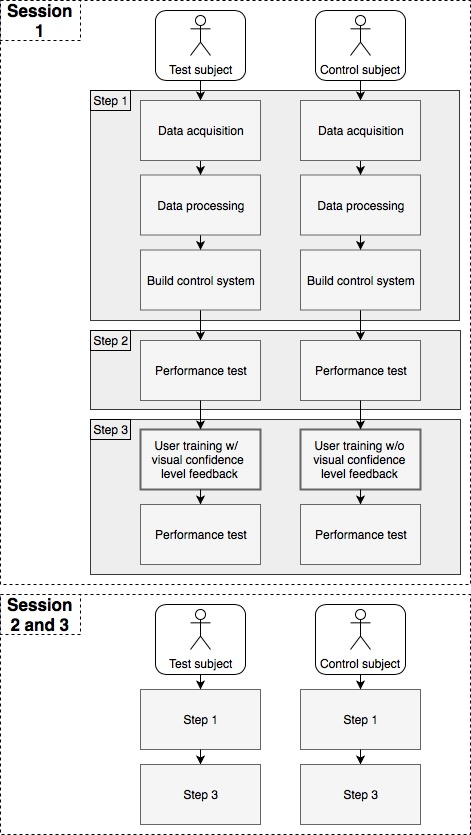
\includegraphics[width=0.42\textwidth]{figures/Paper/Study_design}  
	\caption{Graphical illustration of the experiment showing the steps of each session for the test and control group. Highlighted is user training in step 3 which was the only step that varied between the two groups, and comprised the main area of research interest in the experiment.}
	\label{fig:P:std} 
\end{figure}
\vspace{-0.7cm}
Each subject underwent three sessions; one session per day over three consecutive days. The subjects were randomly allocated to either a test or control group; 8 subjects in each group. During each session EMG signals were initially acquired from the subjects and used to train the control system. The subjects then underwent user training with the purpose of learning how to adapt to the control system. Finally the subjects went through a real time performance test to evaluate their ability to operate a virtual prosthesis. In the first session, the subjects completed the performance test prior to user training. This test was used as a baseline assessment of the subject's performance. All implementations have been performed using MATLAB (2017b). \\
The difference between the test and control groups, and the main area of interest in the study, was in the feedback provided during user training. The test group received the estimated probabilities of each class (confidence scores), while the control group only received label feedback (the estimated class). A flowchart of the study design can be seen in \figref{fig:P:std}.



	
	
	\subsubsection*{Data Acquisition}
	%\subsection{Data acquisition}
EMG signals were recorded with the Myo armband (MYB) from Thalmic Labs - an eight channel dry stainless steel electrode armband. The MYB, which samples at 200 Hz, has a built in 50 Hz notch filter and a Bluetooth 4.0 unit which enables wireless communication with a computer. A 2$^{nd}$ order Butterworth high-pass filter with a 10 Hz cut-off was digitally implemented to reduce movement artefacts. Due to the low sampling with no beforehand low-pass filtering, aliasing of the signal was inevitable, thus no anti-aliasing filter was implemented. Despite the low sampling rate, the MYB has shown to provide EMG recordings that can be classified with significantly similar accuracy as EMG recordings acquired with conventional EMG surface electrodes sampled at 1000 Hz \cite{Mendez2017}. \\
The subjects were instructed to elicit muscle contractions corresponding to the following classes of hand movements: \textit{Wrist extension, Wrist flexion, Radial deviation, Ulnar deviation, Closed hand, Open hand and Rest}, which are illustrated in \figref{fig:P:experiment_movements}. The subjects had their dominant forearm disinfected, and were instructed in wearing the MYB at the thickest part of that forearm. To ensure the same placement of the MYB on each subject, the main electrode-channel was placed most laterally when standing in the anatomical standard position. The subjects were seated on a chair with the dominant arm hanging relaxed laterally down the torso during the whole experiment. \\

According to Scheme et al. \cite{Scheme2015}, the use of dynamically changing contraction data in training a classification-based control scheme has shown to improve performance and tolerance to proportional control. Based on this finding, the subjects performed three repetitions of each movement, where each repetition constituted of a 2.5 second increasing ramp contraction, a 5 second steady state contraction at the peak of the increasing ramp contraction and a 2.5 second decreasing ramp contraction. To assure that each repetition was carried out correctly, the subjects were instructed in tracking a cursor, representing the EMG signal, on a trapezoidal trajectory, where the slopes corresponded to the ramp contractions and the plateau corresponded to the steady state contraction. The plateau of the trajectory differed between the three repetitions as 40 \%, 50 \% and 70 \% of an initial recorded 15 second constant force of Maximum Voluntary Contraction (MVC). Of the recorded time only the plateau phase and the last second on the incline and first second of the decline were used to fit the classifier. To avoid muscle fatigue the subjects were given 30 seconds rest after an MVC recording and 10 seconds rest between repetitions. 

\begin{figure}[H]                 
	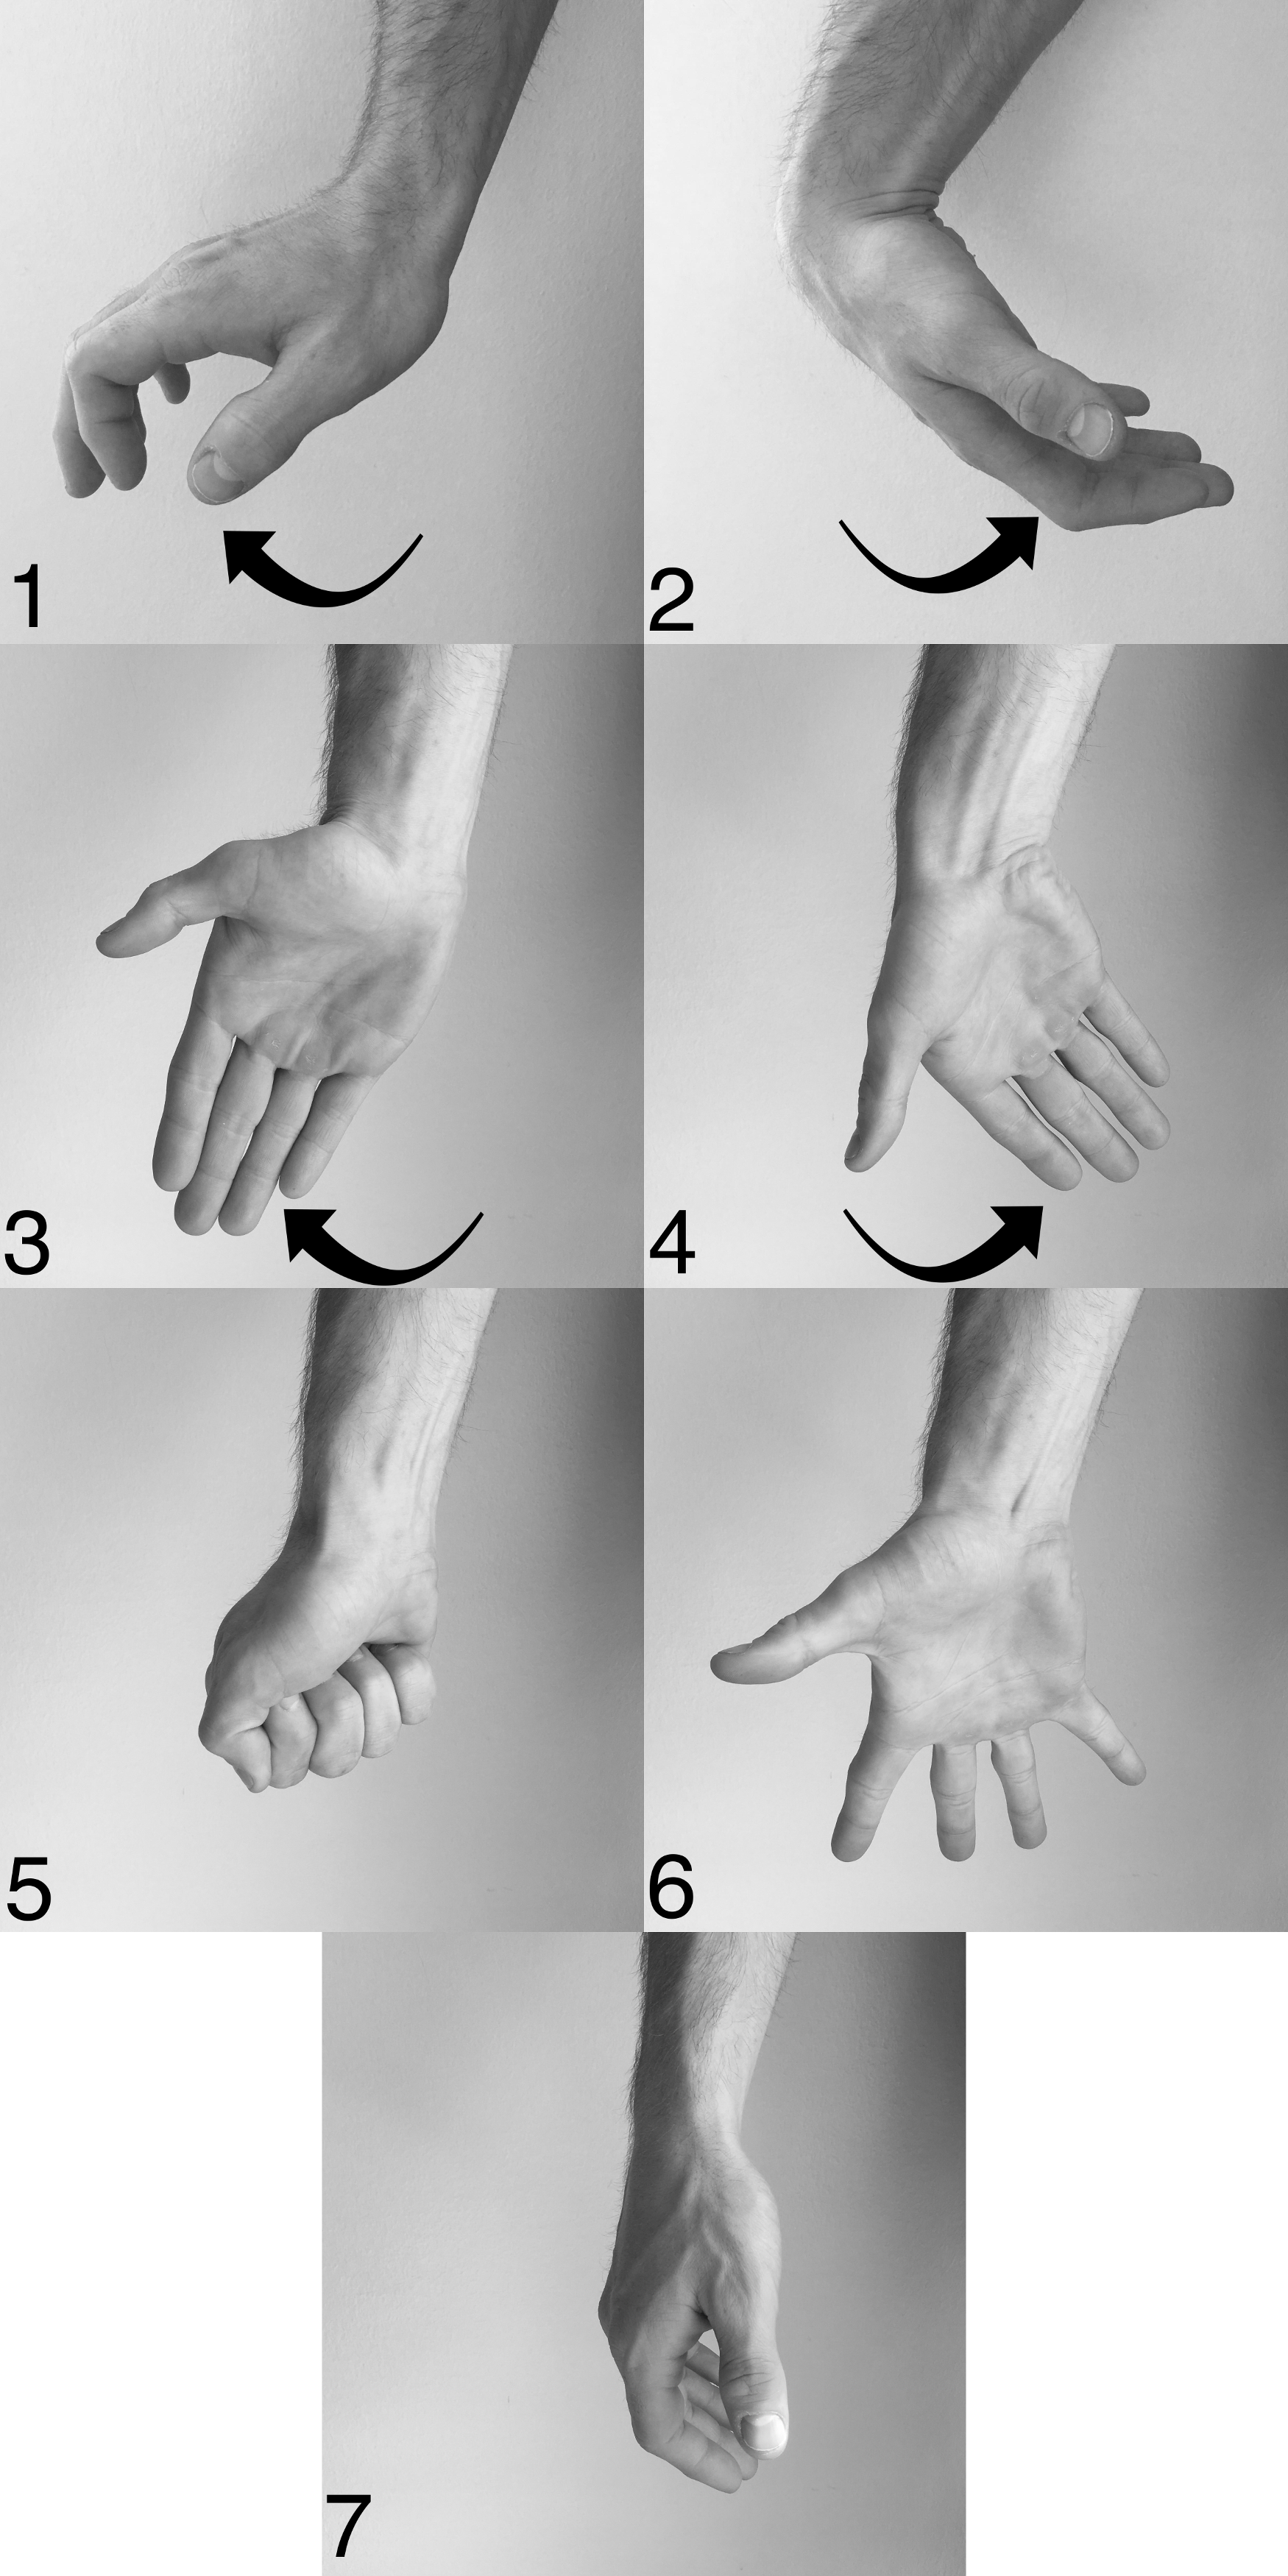
\includegraphics[width=.35\textwidth]{figures/Paper/allHandMovementsVerticalBW}  
	\caption{Illustration of the movements performed in the experiment. 1: Wrist extension, 2: Wrist flexion, 3: Radial deviation, 4: Ulnar deviation, 5: Closed hand, 6: Opened hand, 7: rest.}
	\label{fig:P:experiment_movements} 
\end{figure}
	
%	\subsubsection*{Cluster Dispersion and Separability} 
%	%\subsection{Cluster dispersion and separability}
The EMG signal for each movement class acquired from the subjects forms clusters of multidimensional data points. The lower the dispersion of the individual movement class clusters is, the more distinguishable the movements are, and the classifier will recognize the movement classes with higher accuracy. Additionally, a higher distance between cluster centroids will facilitate a higher classification accuracy further. \\%This section describes how to calculate the cluster dispersion and separability of clusters. \\
To calculate cluster dispersion, the centroid of multidimensional clusters must be calculated as in:

 \begin{equation} \label{eq:centroid}
C = \frac{\sum\limits_{n=1}^{N}a_{n},b_{n},~...~k_{n}}{N}
\end{equation}

Where $C$ is the centroid, $n$ is the number of data points in a dimension, $N$ is the total number of data points in a dimension and $k$ is the number of dimensions. To calculate cluster dispersion, the Euclidean distance (ED) from data point $p$ to the corresponding cluster $q$ is computed: %The ED is the length of the a line segment connecting points, in this case in form of data point $p$ and cluster centroid $q$, and is calculated as:

\begin{equation} \label{eq:euclidiandistance}
ED(p,q) = \sqrt{(p_1-q_1)^2 + (p_2-q_2)^2~+~...~+ (p_k-q_k)^2}
\end{equation} 

Where $p_k$ and $q_k$ are the coordinates of vectors $p$ and $q$ respectively. This procedure is performed for all data points in a cluster, from which the average is calculated to obtain a general impression of the cluster dispersion.\\
To calculate the cluster separability, the ED between cluster centroids is calculated.  
%When calculating the distance from feature values in a cluster to their corresponding centroid the ED is computed likewise. To get a general impression of the distance from the feature values constituting the cluster to the centroid of the cluster the average of the distances is calculated. 


	
	\subsubsection*{Feature Extraction}
	%\section{Feature extraction} 
	
Before training the classifier, features were extracted from the signal. The raw EMG signal from each MYB channel was segmented into 200 ms windows with a 50 \% overlap respecting the findings of Farfán et al. \cite{Farfan2010}. Based on using the MYB for data acquisition recommendations made by Donovan et al. \cite{Donovan2017} regarding the optimal features for low bandwidth sEMG pattern recognition were taken into consideration. These features provided useful signal information even though the MYB only samples sEMG signals with 200 Hz, and in this case offering better accuracy than the Hudgins features \cite{Hudgins1993} in a LDA based control scheme \cite{Donovan2017}. \\
Four space domain (SD) features of Scaled Mean Absolute Value (SMAV), Correlation Coefficient (CC), Mean Absolute Difference Normalized (MADN), Scaled Mean Absolute Difference Raw (SMADR) were used for feature extraction. These features represent a portion of the features Donavan et al. \cite{Donovan2017} proposed, as the rest were left unused due to the intent of reducing feature redundancy. The calculation of SD features lean on the calculation and relation of other SD features. Special for the SD features is utilizing the relation between signals acquired in the different channels of the MYB. Additionally, the well known Hudgins time domain feature Waveform Length (WL) was included to cover complexity information in the time domain \cite{Phiny2012}. The calculation of the features can be found in the appendix. %These features were chosen with the aim of acquiring valuable signal information from both signal amplitude and frequency.  

	
%	\subsubsection*{Confidence Scores} 
%	%\subsection{Confidence scores}
As the application of confidence scores during user training is the main focus of this study, a brief derivation of confidence scores will be presented in this section. This theoretical derivation of confidence scores from a LDA classifier is based on a study by Scheme et al. \cite{Scheme2013}. \\
The decision rule for LDA classification is based on deciding the class with the highest probability of having produced a given input sample. LDA classification is derived from Bayes principles \cite{Scheme2013a}, from which the Bayes theorem expresses that the posterior probability $P(\omega_{j}|x)$, the probability of sample $x$ belonging to class $j$, can be written as:

\vspace{-0.7cm}

\begin{equation}
	P(\omega_{j}|x) = \frac{P(x|\omega_{j})P(\omega_{j})}{P(x)}
\end{equation}
\vspace{-0.02cm}
\noindent Where $P(x|\omega_{j})$ is the class conditional probability, the likelihood that a sample from class $j$ occurs, $P(\omega_{j})$ is the prior probability, the probability of class $j$ occurring, and $P(x)$ is the normalization factor that ensures the probabilities of all class sum to 1. As $P(x)$ is common for all classes, it can be excluded, which leaves the following function:
\vspace{-0.05cm}
\begin{equation} \label{eq:bayeslda}
	g_{j}(x) = P(x|\omega_{j})P(\omega_{j})
\end{equation} 
\vspace{-0.02cm}
\noindent Where $g_{j}(x)$ is a decision boundary. An assumption of LDA is that each class belongs to a Gaussian distribution. Thus, the class conditional probability can be written as the multivariate normal distribution:
\vspace{-0.05cm}
\begin{equation}
P(x|\omega_{j}) = \frac{1}{|\varSigma_{j}|^{1/2}}(\frac{1}{\sqrt{2\pi}})^{d} ~~e^{-1/2} (x-\mu_{j})' ~\varSigma^{-1}_{j} (x-\mu_{j})
\end{equation} 
\vspace{-0.05cm}
\noindent Where $\varSigma_{j}$ and $\mu_{j}$ are the covariance matrices and mean vector for class $j$ and $d$ is the number of dimensions. \\
It can be assumed that all classes share the same covariance matrices $\varSigma$. $\varSigma_{j}$ can thus be replaced with the common covariance matrix $\varSigma$. Through taking the natural logarithm to remove constants, and through mathematical manipulation the function in \eqref{eq:bayeslda} can be written as:
\vspace{-0.05cm}
\begin{equation} 
	g_{j}^{*}(x) = \mu_{j}\varSigma^{-1}x' - \frac{1}{2}\mu_{j}\varSigma^{-1}\mu'_{j} - ln(P(\omega_{j}))
\end{equation}
%\vspace{-0.01cm}
\noindent Which can be written as the linear discriminant classifier:
%\vspace{-1cm}
\begin{equation} \label{eq:ldclassifier}
	g_{j}^{*}(x) = weight_{j}\cdot x' + bias_{j}
\end{equation}
%\vspace{-1cm}
The likelihoods obtained from \eqref{eq:ldclassifier} can be used to calculate the confidence score of a sample belonging to a class $j$. The natural logarithmic operation used to derive $g_{j}^{*}(x)$ transformed the function to the log domain. To calculate the confidence scores the function must be transformed back to the linear domain. Additionally, the class $j$ likelihood must be normalized regarding the sum of all class likelihoods, in order to be a value between 0 and 1, and results in the following calculation of confidence score:
\vspace{-0.05cm}
\begin{equation}
	CS_{k}(x) = \frac{e^{g^{*}_{j}(x)}}{\sum\limits^{J}_{j=1}~e^{g^{*}_{j}(x)}}
\end{equation}
\vspace{-0.05cm}
\noindent Where $CS_{k}(x)$ is the confidence score of a sample $x$ belonging to class $j$. The normalization operation was included to represent the class confidence score as a percentage of the sum of all class confidence scores, in order to have $CS_{k}(x)$ presented as a more intuitive number for the user.
The LDA classifier will be used in the control scheme. To obtain smoother control, the class with the highest average likelihood based on features from the previous three segments is chosen as output class. \\

 
	
	\subsubsection*{Proportional Control}
	%\subsection{Control} \label{sub:P:control}
The LDA classifier described in \subref{sub:P:confidencescores} was used in the control scheme. To obtain more smooth control, the class with the highest average likelihood based on features from the previous three segments was chosen as output class. \\
For proportional control multivariate linear regression models were utilized. One regression model was trained for each movement class (six in total), where the independent variables were Mean Absolute Values (MAV) extracted from each segment in each channel of the MYB. The dependent variables were set as the averaged EMG signal across all channels normalized with the MVC as a reference. Thus, the proportional output value was a single value between 0 and 1. The calculation was as follows: 

\begin{equation} \label{eq:P:multiLinearRegression}
\hat{Y} = \alpha + \beta_1 X_{1} + \beta_2 X_{2} + ... + \beta_i X_{i} + \epsilon_i
\end{equation} 

Where $i$ is the number of MYB channels, $\hat{Y}$ is the proportional control output, $X_{i}$ is the MAV feature of a segment in the $i_{th}$ channel, $\alpha$ is the regression intercept and $\beta$ is the regression slope. Similarly as the classification control, the proportional control output was calculated as the average output from on the three previous segments to obtain smooth control. This control scheme was used in both the user training and the performance test.
	
	\subsubsection*{User Training}
	
%\section{User training}

Subjects were set to train their understanding of making distinguishable hand movements, using a user training interface, where feedback corresponding to the assigned group was presented. Prior to training subjects were informed of the importance of their efforts in relation to the experiment with the intent of encouraging a focused participation. \\
The user training interface contained the following feedback: an illustration of the movement needed to be performed, a horizontal bar visualizing the contraction level and a vertical bar plot visualizing which movement being recognized by the control system. An illustration of the user training interface is shown in \figref{fig:feedbackGUI}. The only difference between test and control group was the type of confidence feedback shown trough the vertical bar plot. 

\begin{figure}[H] 
	\centering
	\subfigure[Test group user training interface.]
	{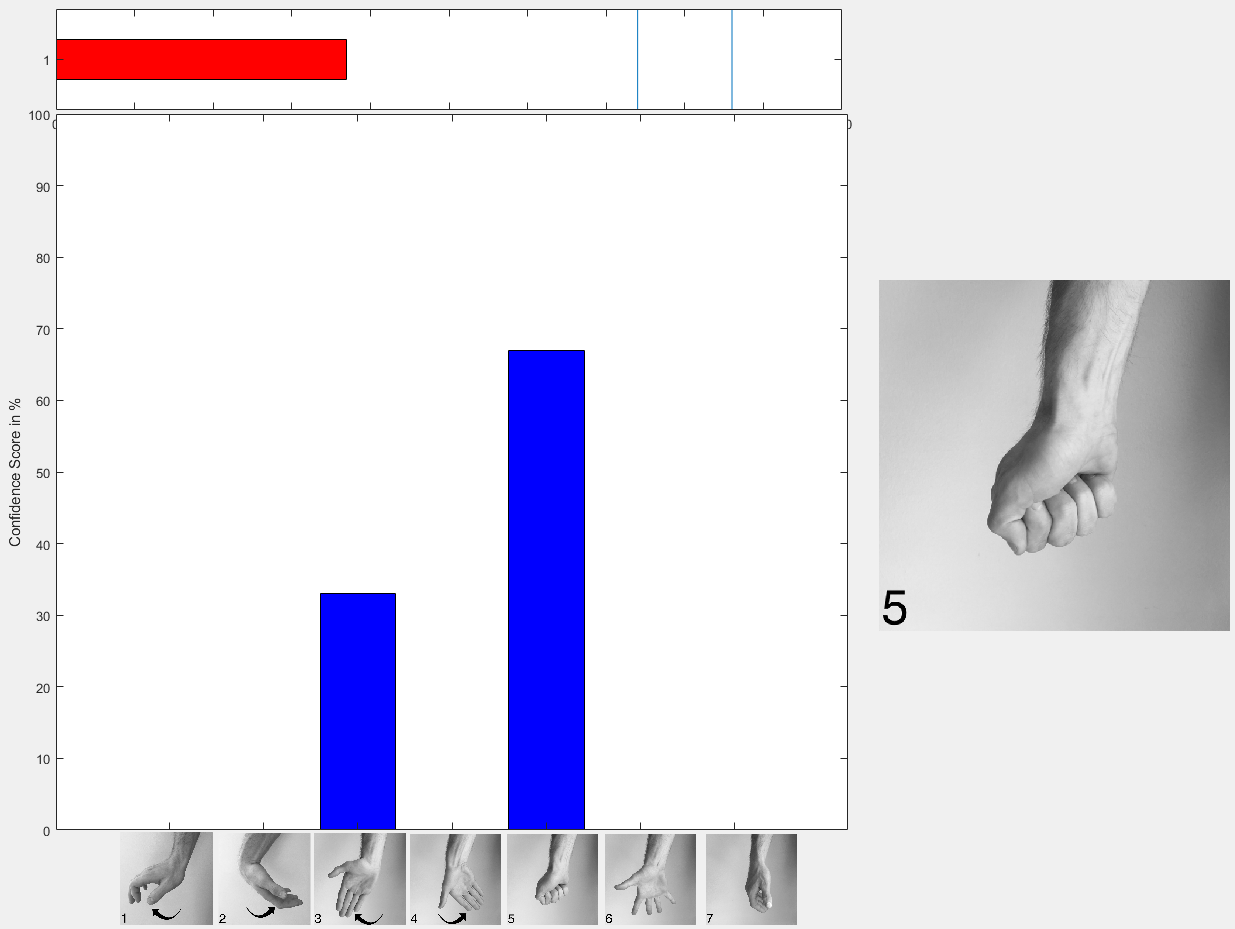
\includegraphics[width=.42\textwidth]{figures/xBackground/usertraintestGUI}} \\
	\subfigure[Control group user training interface.]
	{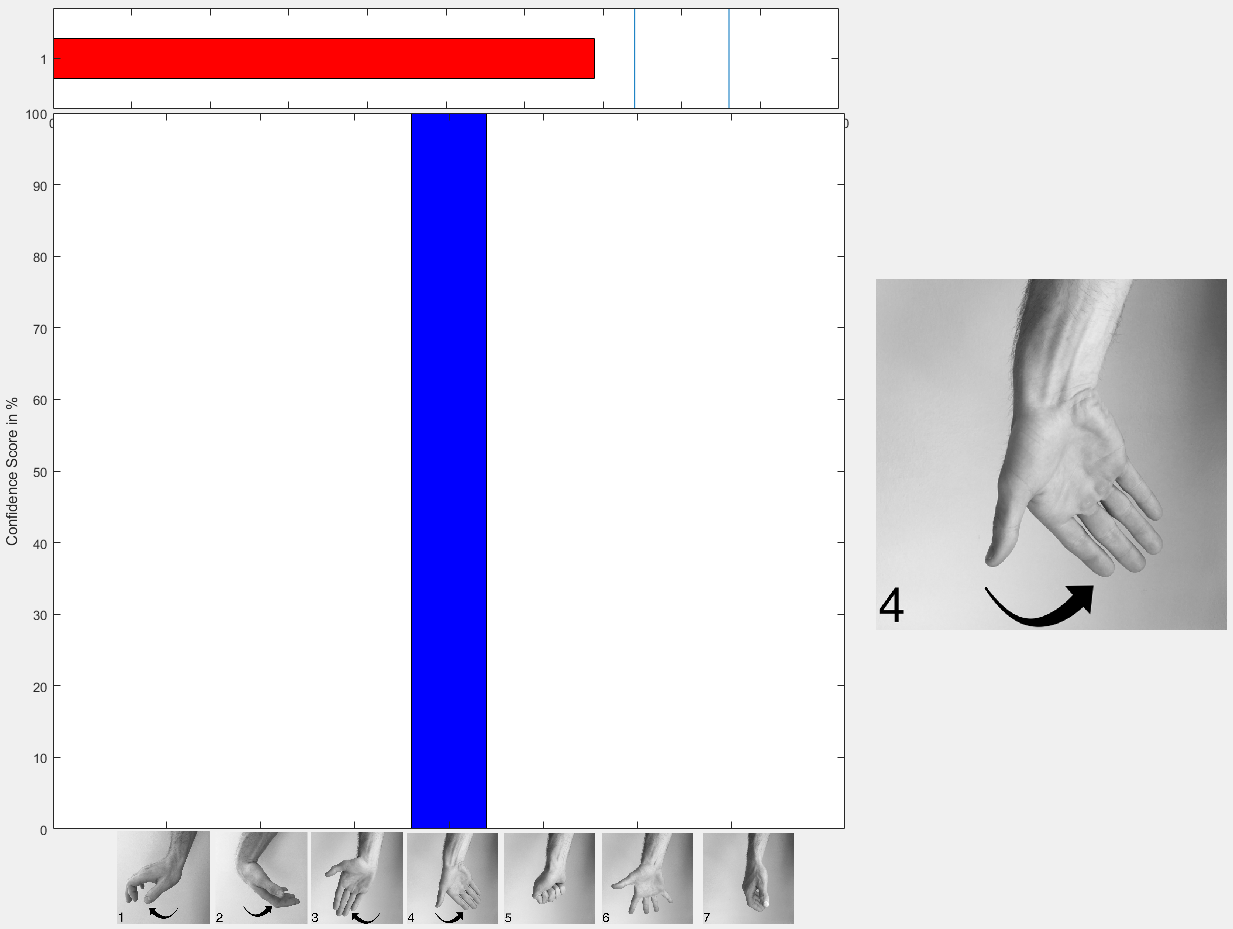
\includegraphics[width=.42\textwidth]{figures/xBackground/usertraincontrolGUI}}  
	\caption{Illustration of the user training interface for the test group (a) and the control group (b). The vertical bar plot indicates which movement is being recognized visualized by the images of each movement; a full bar corresponds to 100 \% recognition confidence. The horizontal bar plot indicates contraction level, where a full bar corresponds to the MVC. The two vertical lines in the contraction level bar plot illustrates the contraction level interval the subject must reach. The large picture of a movement on the right of the bar plot indicates which movement needs to be performed. The difference between the feedback the two subject groups receive is the information given in the vertical recognition bar plot. The control group only sees a full bar of the movement the control system recognizes the most, whereas the test groups receives the exact recognition probabilities of all movements.}
	\label{fig:feedbackGUI}
\end{figure}

The test group was shown the classifier confidence scores for multiple classes, which enabled the possibility of having multiple vertical plots shown. Thus, more diverse feedback was presented, which the user could utilize to correct the performed movement. The control group had only the movement with the highest confidence shown, thereby limiting the confidence feedback to only one bar visible at a time. Thus, the control group was not informed on the exact probabilities of which movements the control system recognized.      


The intent of user training was to train the subject in being more aware of how to perform a movement in a way the classifier would recognize as the movement the user actually performed. To motivate the subject during user training a simple task was implemented in the interface.  The subject had to perform the instructed movement and achieve a minimum of 75\% confidence, whilst also managing to perform the movement within the contraction level interval indicated by the vertical boundaries in the horizontal bar plot. Once these requirements were met and withheld for one second, a sound would appear indicating task completion. The subjects had to return to the rest class and then repeat the movement. The goal was to manage as many repetitions as possible within 30 seconds, then a 10 second break was issued before moving to the next movement. \\
The sequence of a training session were put together in form of the subject having to perform each of the six movements in combination with four different contraction level intervals; 75-85 \%, 55-65 \%, 35-45 \% and 15-25 \% of their MVC. The instructed movements were trained in a random order and the subjects needed to perform all movements in the same contraction level interval before moving to a new interval. This resulted in a total training session time of 16 minutes.         



	
	\subsubsection*{Performance Test}
	%\subsection{Performance test}
A performance test was developed to evaluate the users ability to operate a virtual prosthesis. The test was implemented as a 3D Fitts' Law target reaching test, similar to methods reported in \cite{Scheme2013, Scheme2013a}. The user controlled a circular cursor in a Cartesian coordinate system, where the cursor was to be matched with the appearing targets. Extension/flexion of the wrist moved the cursor horizontally, radial/ulnar deviation moved the cursor vertically and opened/closed hand increased/decreased the size of the cursor. The cursor moved proportional to contraction intensity with a velocity between 0 and 1, where 1 corresponded to the MVC. An illustration of the Fitts' Law test interface can be see in \figref{fig:fittsLawTask}. \\
To reach a target the user had to match the size and position and dwell within the area for 1 second. The target would appear for 15 seconds or until it was reached, after which a new target would appear and the cursor position would be reset to origin. A total of 16 targets would appear before the test ended. The sequence of targets appearing was different between all four test session, to avoid bias of subjects remembering the sequence in which targets would appear. \\


\vspace{-0.2cm}
Originally the Fitts' Law test had a single performance measure, \textit{throughput} (TP) \cite{Fitts1954}. TP uses the relationship between time taken to reach a certain target in seconds ($MT$) and the index of difficulty (ID), and is defined as:
%\vspace{-0.1cm}
\begin{equation} \label{eq:TP}
TP=\frac{1}{N}\sum_{i=1}^{N} \frac{ID_i}{MT_i} 
\end{equation}
%\vspace{-0.1cm}
\noindent Where $i$ is a specific movement and $N$ is the total number of movements. ID relates to the target's width $W$ and distance $D$ from origin, where $W$ and $D$ are unitless. The ID is calculated as: 
%\vspace{-0.1cm}
\begin{equation} \label{eq:ID}
ID=log_2(\frac{D}{W}+1)
\end{equation}
%\vspace{-0.1cm}
\noindent According to \cite{Scheme2013a}, it is in practice most resourceful to use a variety of ID's in a Fitts' Law test. Based on this assumption, the target ID's seen in \tabref{tab:P:ID} were calculated for this study.
\begin{figure}[H] 
	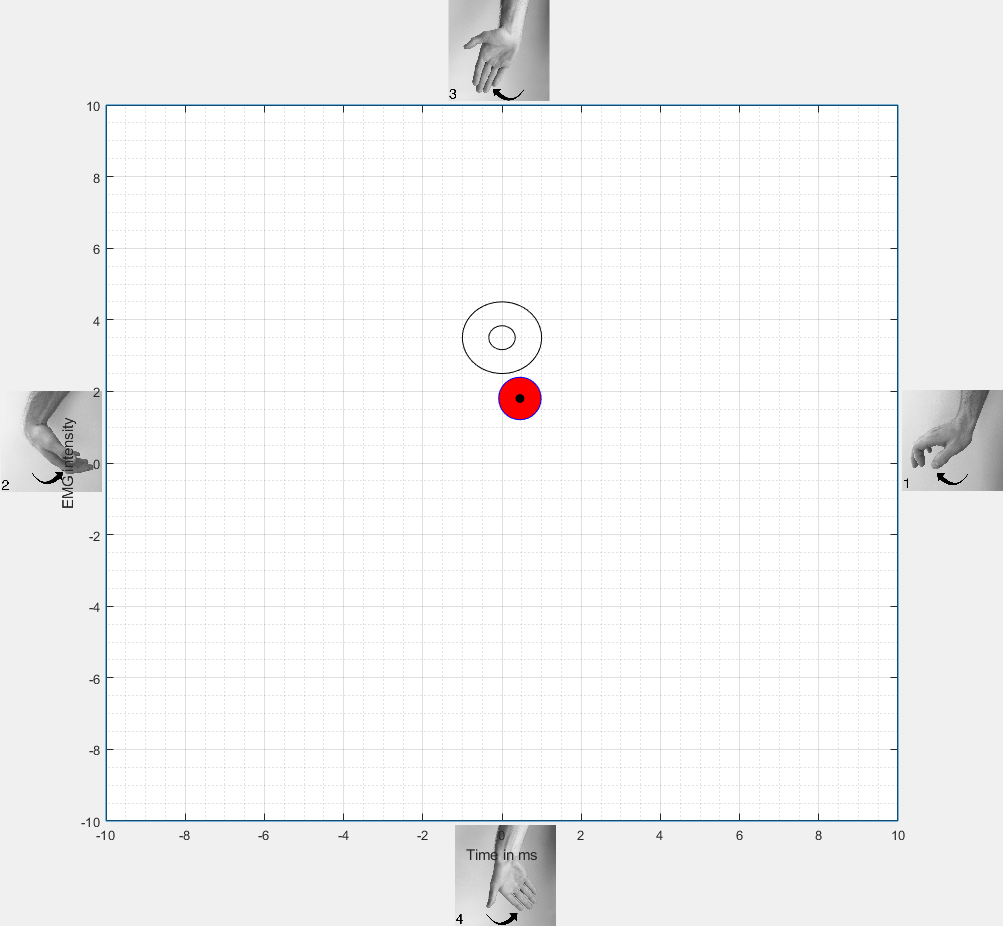
\includegraphics[width=0.49\textwidth]{figures/xBackground/perftestGUI}
	\caption{The implemented interface for the modified Fitts' Law test. The user controlled the red cursor with the centred bold mark. The target consisted of a circle with a larger circle surrounding it. The user was instructed in matching the cursor with the target, where the bold mark should be positioned inside the inner circle of the target, and the outer circle of the cursor should be matched in size with the outer circle of the target. The cursor would then turn green to indicate the matching was correct, and blue when the dwell time was reached.}
	\label{fig:fittsLawTask}
\end{figure}
%\vspace{-1.0cm}
Further performance measures were included similar to previously reported in \cite{Scheme2013, Scheme2013a}. These measures consists of \textit{Path Efficiency}, \textit{Overshoot}, \textit{Stopping Distance} and \textit{Completion Rate}. \\
The additional four measures were added to quantitatively assess performance of naturalness, spontaneity, and compensatory motions during control. The calculation of these features can be found in the appendix. 
\begin{table}[H]
	\centering
	\caption{The index of difficulty used in the Fitts' Law test.}
	\label{tab:P:ID}
	\begin{tabular}{lll}
		
		Distance		 & Width	         & ID				   \\ \hline \hline
		28.0     & 0.33 & 6.41                \\ %\hline \hline
		24.5     & 0.33 & 6.22                \\ %\hline
		22.0     & 0.33 & 6.01                \\ %\hline
		18.5     & 0.33 & 5.82                \\ %\hline
		16.0     & 0.33 & 5.61                \\ %\hline
		13.0     & 0.33 & 5.32                \\ %\hline
		12.5     & 0.33 & 5.27                \\ %\hline
		9.5      & 0.33 & 4.88                \\ \hline \hline
	\end{tabular}
\end{table}

	
	\subsubsection*{Cluster Dispersion and Separability} 
	%\subsection{Cluster dispersion and separability}
The EMG signal for each movement class acquired from the subjects forms clusters of multidimensional data points. The lower the dispersion of the individual movement class clusters is, the more distinguishable the movements are, and the classifier will recognize the movement classes with higher accuracy. Additionally, a higher distance between cluster centroids will facilitate a higher classification accuracy further. \\%This section describes how to calculate the cluster dispersion and separability of clusters. \\
To calculate cluster dispersion, the centroid of multidimensional clusters must be calculated as in:

 \begin{equation} \label{eq:centroid}
C = \frac{\sum\limits_{n=1}^{N}a_{n},b_{n},~...~k_{n}}{N}
\end{equation}

Where $C$ is the centroid, $n$ is the number of data points in a dimension, $N$ is the total number of data points in a dimension and $k$ is the number of dimensions. To calculate cluster dispersion, the Euclidean distance (ED) from data point $p$ to the corresponding cluster $q$ is computed: %The ED is the length of the a line segment connecting points, in this case in form of data point $p$ and cluster centroid $q$, and is calculated as:

\begin{equation} \label{eq:euclidiandistance}
ED(p,q) = \sqrt{(p_1-q_1)^2 + (p_2-q_2)^2~+~...~+ (p_k-q_k)^2}
\end{equation} 

Where $p_k$ and $q_k$ are the coordinates of vectors $p$ and $q$ respectively. This procedure is performed for all data points in a cluster, from which the average is calculated to obtain a general impression of the cluster dispersion.\\
To calculate the cluster separability, the ED between cluster centroids is calculated.  
%When calculating the distance from feature values in a cluster to their corresponding centroid the ED is computed likewise. To get a general impression of the distance from the feature values constituting the cluster to the centroid of the cluster the average of the distances is calculated. 


	
	\subsubsection*{Statistical Analysis}
	Statistics were applied to evaluate improvements in the results obtained in the performance test, user training and data clustering. A Friedmans test was used for multiple comparison and a Tukey-Kramer correction was conducted when detecting an effect. For comparison between groups in each session, a Mann-Whitney U test was applied.
	
	\section*{IV. RESULTS}%%%%%%%%%%%%%%%%%%%%%%%%%%%%%%%%%%%%%%%%%%%%%%%%%%%%%%%%%%%%%%%%%%%
	
Statistics were applied to evaluate improvements in the results obtained in the performance test, user training and data clustering. A Friedmans test was used for multiple comparison and a Tukey-Kramer correction was conducted when detecting an effect. For comparison between groups in each session, a Mann-Whitney U test was applied. 

\subsubsection*{Performance Evaluation} \label{sec:R:fitts}
This section presents the results acquired from the Fitts' Law target reaching test. The test had five measures which each expresses a parameter of subjects' performance. %Subjects were divided into two groups, one test group which received exact class confidence scores during user training, and a control group which only received a single class confidence score. 
The plotted mean and standard deviations of each measure for all subjects in each group in the performance test for each session can be seen in \figref{thereIsnoFigRefYet}.

\end{multicols}

%throughput
\begin{figure}[H] 
	\subfigure[]
	{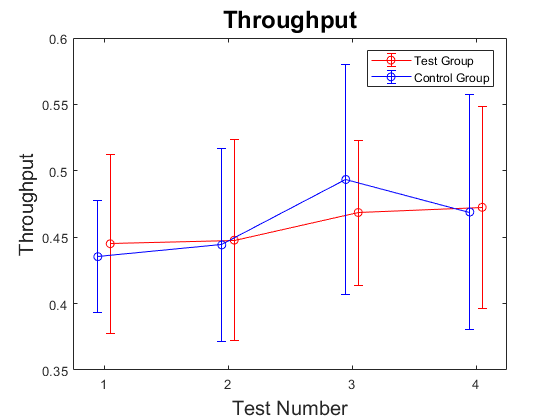
\includegraphics[width=.33\textwidth]{figures/xWesulds/Throughput}} 
	\hspace{-0.5cm}
	\subfigure[]
	{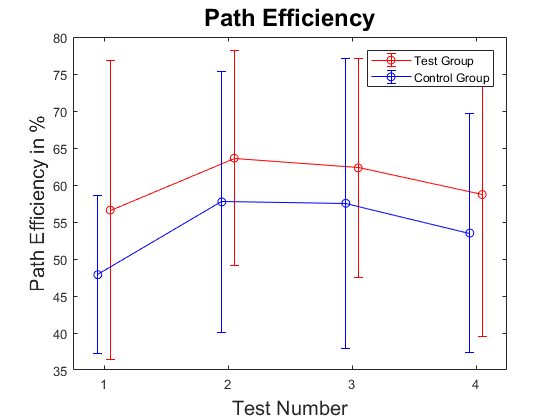
\includegraphics[width=.33\textwidth]{figures/xWesulds/PathEfficiency}} 
	\hspace{-0.5cm}
	\subfigure[]
	{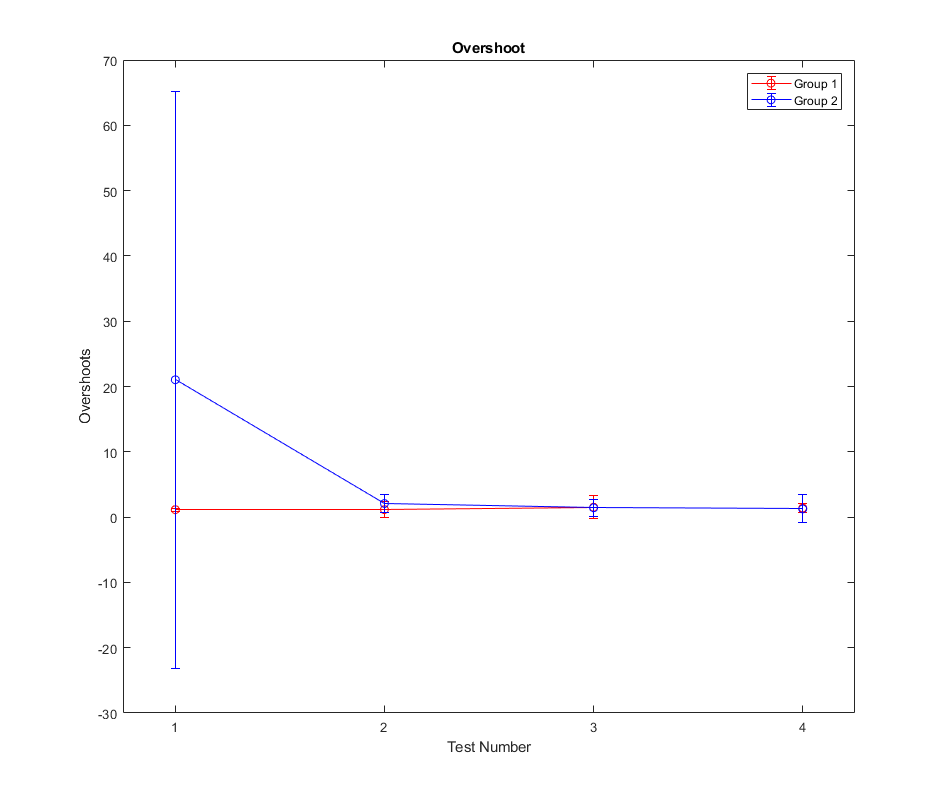
\includegraphics[width=.33\textwidth]{figures/xWesulds/Overshoot}}  
	\subfigure[]
	{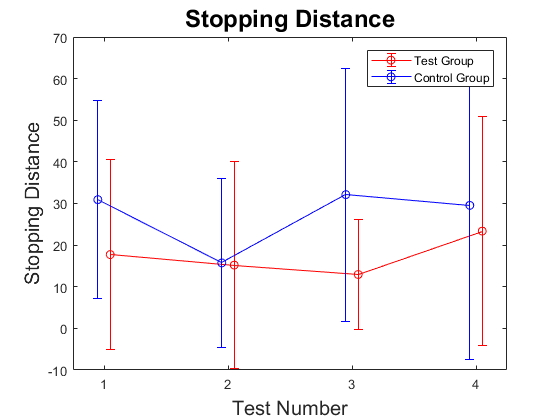
\includegraphics[width=.33\textwidth]{figures/xWesulds/StoppingDistance}} 
	\hspace{-0.5cm}
	\subfigure[]
	{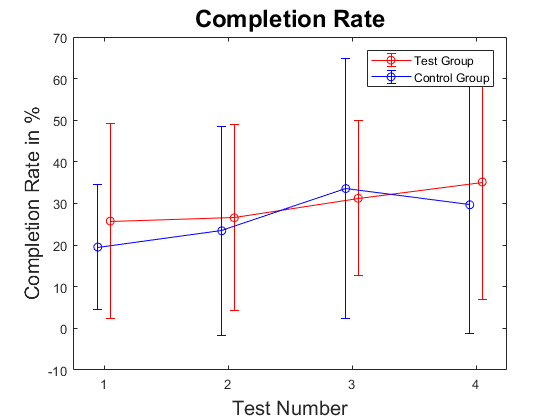
\includegraphics[width=.33\textwidth]{figures/xWesulds/CompletionRate}}  
	\hspace{-0.5cm}
	\caption{Figure illustrating the five performance measures; \textit{ a) Throughput, b) Path efficiency, c) Overshoot, d) Stopping distance, e) Completion rate}, used for quantifying user performance across all four tests. Test number 1 is the acquired baseline used for assessing group homogeneity and the following numbers indicate performance test results after user training in each session. The red line indicates the progression of the test group and the blue line the progression of the control group.}
	\label{thereIsnoFigRefYet}

\end{figure}



%
%%Path Efficiency
%\begin{figure}[H] 
%	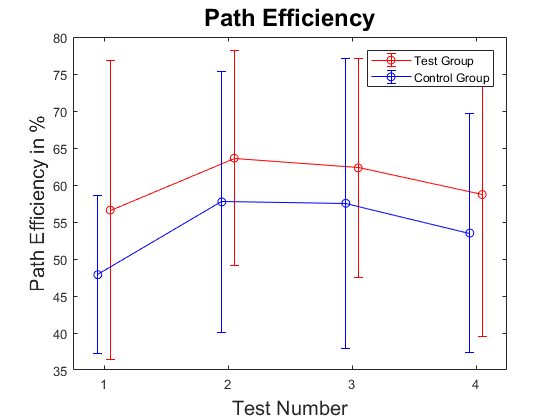
\includegraphics[width=0.3\textwidth]{figures/xWesulds/PathEfficiency}
%	\caption{Path efficiency metric for the Fitts' Law test between the test and control group.}
%	\label{fig:PEresult}
%\end{figure} 
%
%overshoot
%\begin{figure}[H] 
%	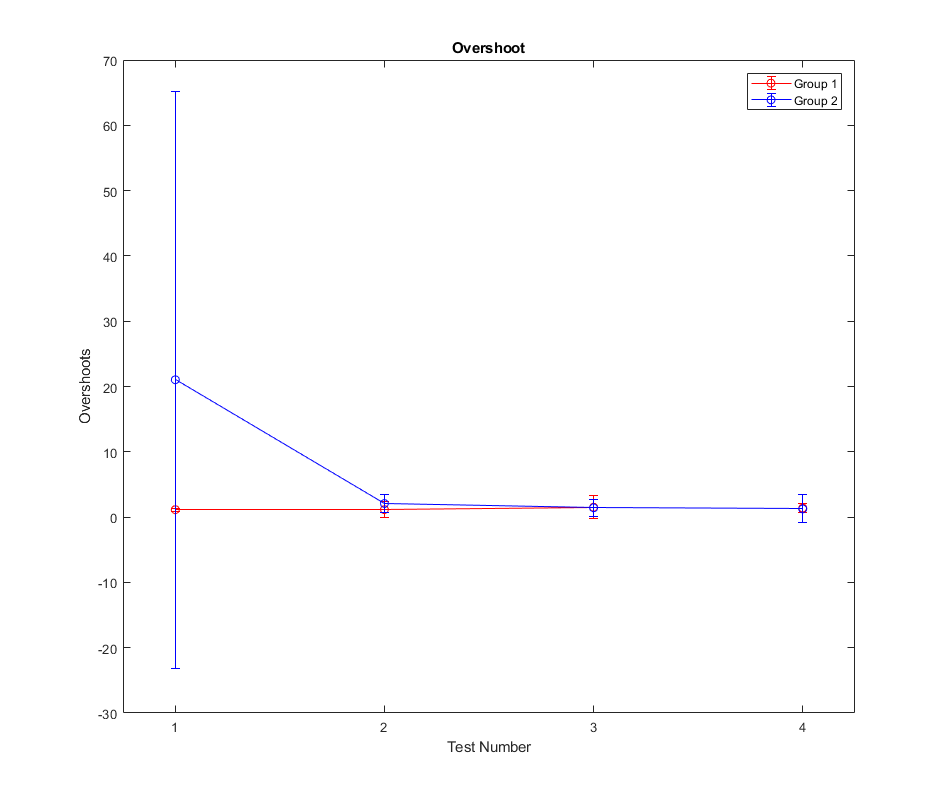
\includegraphics[width=0.3\textwidth]{figures/xWesulds/Overshoot}
%	\caption{Overshoot metric for the Fitts' Law test between the test and control group. There is no significant difference between the groups ($p > 0.05$).}
%	\label{fig:OSresult}
%\end{figure} 

%stopping distance
%\begin{figure}[H] 
%	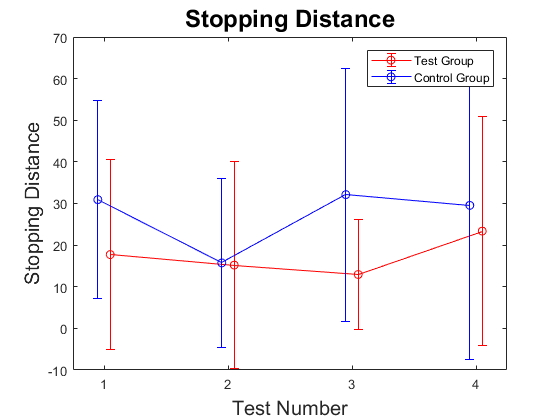
\includegraphics[width=0.3\textwidth]{figures/xWesulds/StoppingDistance}
%	\caption{Stopping distance metric for the Fitts' Law test between the test and control group. There is no significant difference between the groups ($p > 0.05$).}
%	\label{fig:SDresult}
%\end{figure} 
%
%%completion rate
%\begin{figure}[H] 
%	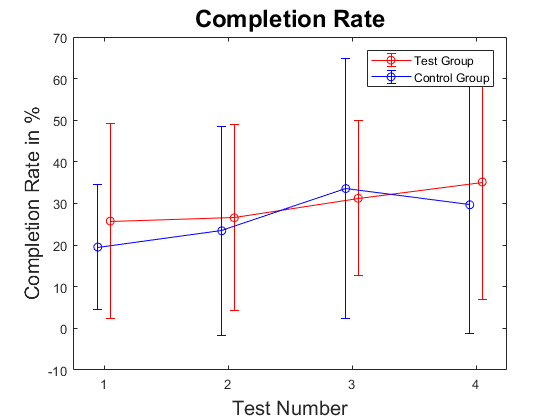
\includegraphics[width=0.3\textwidth]{figures/xWesulds/CompletionRate}
%	\caption{Completion rate metric for the Fitts' Law test between the test and control group. There is no significant difference between the groups ($p > 0.05$).}
%	\label{fig:CRresult}
%\end{figure} 
\begin{multicols}{2}

The baseline performance test showed no difference between the two group, showing the two groups to be homogeneous at initiation. The Fitts' Law test results did not show any significant improvement over the three sessions for any of the five test measures for both the test and control group ($p > 0.05$). Similarly, there was no significant difference between the two groups performance in any sessions ($p > 0.05$), meaning neither of them performed significantly better than the other group in any of the sessions.

\subsubsection*{User Training Evaluation} \label{sec:R:userTraining}

This section covers the results acquired from measurements obtained during user training sessions. During user training subjects were instructed to train movements in being performed such that the control system recognized the movement as the actually performed movement. During this training the number of times subjects correctly performed an instructed movement to the contraction interval shown in the training interface was recorded, and will be referred to at the number of repetitions. \\
No significant difference in the total number of repetitions was found between sessions of either group ($p > 0.05$). When comparing the total number of repetitions of each session between groups accordingly, no significant difference were found either ($p > 0.05$). \\ %During user training the total completion rate is defined by the number of times a subject correctly performed a movement and held the contraction bar at the given interval for one second. A p-value of $p > 0.05$ was found for both groups in the Friedmans test comparing the performance over the three sessions, and Tukey-Kramer correction did not show any significant difference between any of the sessions ($p > 0.05$), which means there was no significant development of performance in the training for any group. 
An increased ability to get repetitions in the low intensities was found for the control group ($p < 0.05$, session 1 $ = 16.13 \pm 5.59$, session 3 $= 21.38 \pm 6.78$). Otherwise, similar results were yielded for both groups when comparing the subjects' ability to reach the three other contraction levels between sessions ($p > 0.05$).\\
%Friedmans test was applied to examine if there was a development in the ability to reach the different contraction levels within the three training sessions. A p-value of $p > 0.05$ was found for both groups, with the Tukey-Kramer correction yielding $p > 0.05$ for the comparison of the three sessions, meaning there was no change in ability to reach different intensities.
No difference was found, when comparing the two groups' ability to reach different intensities during training either ($p > 0.05$).
Comparing the ability to perform different movements during the training showed a significant improvement for the test group in ulnar deviation ($p < 0.05$, session 1 $ = 11.38 \pm 4.27$, session 3 $= 16.13 \pm 2.95$) and open hand ($p < 0.05$, session 1 $ = 11.25 \pm 3.85$, session 3 $ = 17.88 \pm 2.46$). A significant decrease in performance was found for the control group's ability to perform flexion ($p < 0.05$, session 2 $ = 16.63 \pm 2.77$, session 3 $ = 11.00 \pm 3.16$). Otherwise, no significant difference between the three sessions for the two groups was found ($p > 0.05$).\\ %, with the Tukey-Kramer correction resulting in $p > 0.05$ between all sessions for both the test and control group, meaning there was no development in ability to reach specific positions. 
A significant difference ($p < 0.05$) was found between the test and control groups ability to reach the closed hand movement, with a mean of $26.8 \pm13.5$ number of repetitions for the test group and $38 \pm12.2$ for the control group. No significant difference was found for any of the other movements when comparing the two groups ($p > 0.05$).

\subsubsection*{Cluster Dispersion and Separability Results}
In this section results from the data acquisition are presented. The data used for training the LDA based classifier was examined. Each movement resulted in a cluster of data points, which was examined in order to analyse the change in cluster dispersion and distance between cluster centroids.
For both groups the mean distance between the cluster centroids were calculated. The change in between cluster distances over the three sessions were tested and showed no significant difference ($p > 0.05$). Likewise, no significant difference in the development of cluster distances between the groups was found ($p > 0.05$).\\
The mean distance from data points to the cluster centroid was calculated. This showed no significant difference for the test group ($p > 0.05$), but a significant difference was found for the control group ($p < 0.05$). The Tukey-Kramer correction showed the significant difference was between session one and three ($p < 0.05$), where the mean for session one was $502.02 \pm 274.88$, and session three was $323.43 \pm 171.13$. The comparison between groups showed that the control group achieved a significant improvement of within cluster distances compared to the test group in session three ($p < 0.05$), where the test group had a mean distance within clusters of $584.34 \pm 250.02$, while the control group had $323.43 \pm 171.13$. 
%\end{multicols}
	
	
	%\begin{multicols}{2}
	\section*{V. DISCUSSION}%%%%%%%%%%%%%%%%%%%%%%%%%%%%%%%%%%%%%%%%%%%%%%%%%%%%%%%%%%%%%%%%
	
	The results showed no significant difference between the test and control group within the Fitts' Law test, with all comparisons between and within groups yielding p-values below 0.05. This means that none of the groups performed better than the other, and that neither of them managed to improve significantly during the three days of training and testing. The only significant difference ($p < 0.05$) between the groups were found in the training when performing the closed hand gesture, where the test group performed worse than the control group. This difference could be the result of either the training type or the number of subjects.

A main cause of the lacking development within the groups can be the result of a high ID compared to other studies. Several subjects had problems reaching any targets at all, and if the subject was unable to reach any targets, all the Fitts' Law measures except for CR could not be used in the statistical tests. This leads to problems when examining the results, as it was expected that the statistical differences would primarily be found when looking at other measures than CR, as they would offer better insight into the development of the precision when completing the test. 

At the same time a high ID led to subjects becoming frustrated when they had a hard time reaching targets. When overseeing the test it was clear that this frustration resulted in the subjects forgetting how to perform precise movements, which then again led to more frustration. This factor could also have had an effect on the subjects performance. Visible improvement in development of movement precision might also take more than three sessions, and this could also be a cause of the lacking development within the subjects. When developing the understanding of precision there should also be a higher focus on rest, as this is a crucial part of the target test. Some of the subjects did not understand the importance of getting back to rest in training, which might be reflected in the target test.

\subsection{Optimization of Study}
The above points should be taken into consideration when examining the use of uncertainty and confidence scores in training to improve performance further on. When building the system the ID should be adjusted so that in the test it is rather easy to get a CR of 80\% to 100\%, in order to focus on the precision of the control, which is shown better in the other Fitts' Law measures. At the same time a lower ID would give the subjects a feeling of success rather than frustration when performing the test, which might encourage them to retain the interest and focus when training and testing

Furthermore the target test should be developed in a way so that the position and movement from trying to reach a previous target can not affect the position when a new target appears in order to make the test equal for all subjects. At the same time the subjects should be forced to get back to rest in training in order to be able to stay still within a target in the test. This was not implemented in the current training interface, but the importance of learning to rest when using classifiers could be examined in further studies.

When doing further testing the number of sessions should be more than three, and a study to examine the time it takes to improve could be performed in order to find the minimum number of days it takes to achieve higher precision when performing specific hand gestures. The three days of training and testing did not result in a significant performance, but it can be hypothesised that a week of testing might be sufficient to achieve a better control. At last a higher number of test subjects could result in a better distribution within the groups, as some subjects were able to get close to 100 \% CR in the first or second try, while others struggled with reaching just one target. 

\subsection{Other Findings}
While examining the EMG data it was found that the within cluster distance between the centroid and the samples improved within the control group ($p < 0.05$) between the sessions. When applying a Tukey-Kramer correction it was found that the difference was between the first and third session ($p < 0.05$) where the mean distance improved from $502.02 \pm 274.88$ to $323.43 \pm 171.13$. This result shows that the control group became better at performing precise movements, as the EMG data was more closely clustered after training for the three sessions. 

Furthermore a significant difference ($p < 0.05$) was found when comparing the within cluster distance of the two groups, where the mean distance for the control group ($323.43 \pm 171.13$) was close to half of the distance within the test group ($584.34 \pm 250.02$). This could lead to the conclusion that the control group became better at performing the exact movements during data acquisition when compared to the test group, as there was no significant difference when comparing data in the other sessions. 


	
	\subsection*{VI. CONCLUSION}%%%%%%%%%%%%%%%%%%%%%%%%%%%%%%%%%%%%%%%%%%%%%%%%%%%%%%%%%%%%%%%
	
	Based on the results in the experiment it was found that training the user with confidence score feedback compared to label feedback can not be linked to any significant improvement in performance evaluated through a Fitts' Law test. Furthermore, no significant improvement during a three day training period for either the control or the test group was detected. These findings are most likely due to the high index of difficulty, making it hard to draw any conclusions based on the Fitts' Law test. 

Contrarily, it appears that training the user with label feedback can lead to a closer clustering of EMG data compared to training with confidence score feedback. This can be assessed, as a significant improvement was found between the first and last dataset recorded for the control group. To further support this the EMG signal of the subjects who received label feedback clustered significantly closer than the test group on the last day of testing. This shows that training based on confidence scores might not be a way to improve performance, which should be examined further by the use of Fitts' Law tests with lower ID's and a higher number of training sessions. 
	
	%%%%%%%%%%%%%%%%%%%%%%%%%%%%%%%%%%%%%%%%%%%%%%%%%%%%%%%%%%%%%%%%%%%%%%%%%%%%%%%%
	
	
	\subsection*{ACKNOWLEDGMENT}
	
	The authors would like to thank supervisors Strahinja Dosen, Jakob Lund Dideriksen and Lotte N.S. Andreasen Struijk for providing constructive feedback, and the School of Medicine and Health at Aalborg University for providing equipment and the facilities to complete this study. Additionally, the authors are very thankful for all the voluntary participants. 


\renewcommand*{\bibfont}{\footnotesize}
	\urlstyle{same}
	\printbibliography
	
		\section*{VII. APPENDIX}%%%%%%%%%%%%%%%%%%%%%%%%%%%%%%%%%%%%%%%%%%%%%%%%%%%%%%%%%%%%%%%%
		%appendix

%this is appendix
\textbf{Features} \\
In this section the equations used for calculating the features used in this project. \\
MAV is a feature that primarily is affected by the force produces when making a contraction. MAV is extracted for each window and calculated for each of the $i^{th}$ channel. The extraction is expressed as:

\begin{equation} \label{eq:MAV}
MAV_i=\frac{\sum\limits_{n=1}^{ws}|x_i[n]|}{ws}
\end{equation}

where $ws$ is the window size, the number of raw data points in that exact window. $x_i[n]$ is the $n^{th}$ raw data points from the $i^{th}$ channel.  

The mean MAV across all channels, MMAV, is used to remove dependency of movement intensity. MMAV is calculated by using the MAV of all channels for the current window, and is done as following: 

\begin{equation} \label{eq:MMAV}
MMAV=\frac{\sum\limits_{i=1}^{8}MAV_i}{8}
\end{equation}

MMAV can be used to scale the MAV feature creating the SMAV feature. This feature should represent a non-dimensional relationship between channels. SMAV is simply calculated as:

\begin{equation} \label{eq:SMAV}
SMAV_i=\frac{MAV_i}{MMAV}
\end{equation}

As each of the eight EMG sensors in the MYB are located around the arm, they acquire signals from a mixture of sources. Also individual sources may affect multiple sensors depending on their size. Due to this a source measured by multiple sensors will effect their acquired signal correlation. An idea is therefore to calculate the correlation coefficient between each channel and its neighboring channel.  

\begin{equation} \label{eq:CC}
CC_i=\frac{\sum\limits_{n=1}^{ws}X_i[n]X_{i+1}[n]}{ws}
\end{equation}

$X_i[n]$ is the $n^{th}$ normalized data point from channel $i$. When calculating CC the data from each window is normalized by subtracting its mean value from each raw data point, and afterwards divided by their standard deviation. 

Calculating CC can prove rather demanding in computational power due to the series og multiplication operations. Therefore Donovan et al. \cite{Donovan2017} proposed introducing a mean absolute difference-based feature of lower computational complexity which still characterizes the spatial relationship between channels. The MAD feature is normalized in the same way as CC, making up the MADN feature calculated as: 

\begin{equation} \label{eq:MADN}
MADN_i=\frac{\sum\limits_{n=1}^{ws}|X_i[n]-X_{i+1}[n]|}{ws}
\end{equation}

If the normalization of the signal proves too demanding the feature can be calculated on the raw EMG-signal without the normalization. This makes up the MADR feature, calculated as:

\begin{equation} \label{eq:MADR}
MADR_i=\frac{\sum\limits_{n=1}^{ws}|x_i[n]-x_{i+1}[n]|}{ws}
\end{equation}

As the SMAV feature the MAD feature can be scaled by MMAV to remove movement intensity dependency. SMADR is calculated for each channel by:

\begin{equation} \label{eq:MMADR}
SMADR_i=\frac{MADR_i}{MMAV}
\end{equation}


As stated in the beginning some of these features introduce redundancy, subsequently the features of SMAV, CC, MADN and SMADR are the ones used for classification. \cite{Donovan2017}

To further improve the decision foundation of the classifier it was proposed to include the time domain feature of WL calculated by: 

\begin{equation} \label{eq:WL}
WL_i=\sum\limits_{n=1}^{N-1}|x_{i+1}[n]-x_i[n]|
\end{equation}

WL is a measure of the signal complexity by calculating the cumulative length for each channel \cite{Phiny2012}.




\textbf{Fitts' Law Measures} \\
In this section the equations for the Fitts' Law measures are presented. \\
Throughput (TP) which represents the trade-off between speed and accuracy. TP uses the relationship of time taken to reach a certain target in seconds ($MT$) and the index of difficulty (ID). This forms: \cite{Scheme2013,Fitts1954}

\begin{equation} \label{eq:TP}
TP=\frac{1}{N}\sum\limits_{i=1}^{N} \frac{ID_i}{MT_i} 
\end{equation}

where $i$ is a specific movement and $N$ is the total number of movements. ID relates to the target distance $D$ and width $W$. The ID for each task, from the origin to a specific target of a certain size is calculated using \cite{Scheme2013,Fitts1954}:

\begin{equation} \label{eq:ID}
ID=log_2(\frac{D}{W}+1)
\end{equation}

Path Efficiency (PE) describes the quality of control by making a measure of the straightness of the cursor's path to the target, by making a ratio of the actual path distance versus the optimal path distance. This tests the users ability to continuously control the cursor position. Following the optimal path will result in a PE of 100\%. PE is calculated as follows \cite{Scheme2013, Poulton2013}:       

\begin{equation} \label{eq:PE}
PE = \frac{Optimal ~ Distance}{Actual ~ Distance}
\end{equation}		 

Overshoot (OS) is the number of times the cursor enters and then leaves the target before the dwell time inside the target is reached, across all target in the task, divided by the total number of targets. OS tests the users ability to control the velocity of the cursor accurately. A perfect OS-score of zero is reached if the cursor dwells within the target boundaries on the first try for all targets, and is calculated as the following \cite{Scheme2013, Poulton2013}:

\begin{equation} \label{eq:OS}
OS = \frac{Total ~ Number ~ of ~ Overshoots}{Total ~ Number ~ of ~ Targets}
\end{equation}

Stopping Distance (SD) describes the users ability to rest and thereby perform no movement. The SD measure is the distance moved during the dwell time across all targets, and is given as \cite{Scheme2013}:

\begin{equation} \label{eq:SD}
SD = \sum\limits_{i=1}^{N} (Distance ~ Inside ~ Target)_i
\end{equation}

where $i$ is a reached target and $N$ is the total number of reached targets.

Completion Rate (CR) describes the percentage of targets reached within the total allowed time. This gives a general idea of the user's performance, and is calculated as \cite{Scheme2013,Simon2011}: 

\begin{equation} \label{eq:CR}
CR = \frac{Number ~ of ~ Reached ~ Targets}{Total ~ Number ~ of ~ Targets}
\end{equation}
	
	%			\bibitem{citeKey} author, title, publisher , volume, year
	
	%	\begin{thebibliography}{99}				
	%		\bibitem{Fougner2012} Fougner, Anders and Stavdahl, Oyvind and Kyberd, Peter J. and Losier, Yves G. and Parker, Philip A., Control of upper limb prostheses: Terminology and proportional myoelectric control a review, IEEE Trans. Neural Syst. Rehabil. Eng., 20, 2012
	%		\bibitem{amsuess2014} Amsuess, Sebastian and Goebel, Peter and Graimann, Bernhard and Farina, Dario, Extending mode switching to multiple degrees of freedom in hand prosthesis control is not efficient, 2014
	%		\bibitem{Ison2016} Ison, M and Vujaklija, I and Whitsell, B and Farina, D, High-density electromyography and motor skill learning for robust long-term control of a 7-DoF robot arm, IEEE Trans., 24, 2016
	%		\bibitem{hahne2014} Hahne, J. M. and Biebmann, F. and Jiang, Ning and Rehbaum, Hubertus and Farina, Dario and Meinecke, F. C. and Muller, K.-R and Parra, L. C., Linear and Nonlinear Regression Techniques for Simultaneous and Proportional Myoelectric Control, IEEE Trans. Neural Syst. Rehabil. Eng., 22, 2014
	%		\bibitem{jiang2010} Jiang, Ning and Vujaklija, Ivan and Rehbaum, Hubertus and Graimann, Bernhard and Farina, Dario, Is accurate mapping of EMG signals on kinematics needed for precise online myoelectric control?, IEEE Trans. Neural Syst. Rehabil. Eng., 22, 2014
	%		\bibitem{jiang2012} Jiang, Ning and Dosen, Strahinja and Muller, K R and Farina, Dario, Myoelectric Control of Artificial Limbs: Is There a Need to Change Focus?, IEEE Signal Process. Mag., 29, 2012
	%		\bibitem{Fougner2011} Fougner, Anders and Scheme, Erik and Chan, Adrian D.C. and Englehart, Kevin and Stavdahl, {\O}yvind, Resolving the limb position effect in myoelectric pattern recognition, IEEE Trans. Neural Syst. Rehabil. Eng., 19, 2011
	%		\bibitem{DeRugy2012} de Rugy, A. and Loeb, G. E. and Carroll, T. J., Muscle Coordination Is Habitual Rather than Optimal, J. Neurosci., 32, 2012
	%		\bibitem{jiang2009} Jiang, Ning and Englehart, Kevin B. and Parker, Philip A., Extracting simultaneous and proportional neural control information for multiple-dof prostheses from the surface electromyographic signal, IEEE Trans. Biomed. Eng., 56, 2009
	%		\bibitem{Roy2010} Roy, Serge H and Cheng, M Samuel, A Combined sEMG and Accelerometer System for Monitoring Functional Activity in Stroke, Vital Heal. Stat. Ser. 20, 17, 2010
	%		\bibitem{Imtiaz2014} Imtiaz, U. and Yamamura, K. and Kong, W. and Sessa, S. and Lin, Z. and Bartolomeo, L. and Ishii, H. and Zecca, M. and Yamada, Y. and Takanishi, A., Application of wireless inertial measurement units and EMG sensors for studying deglutition - Preliminary results, Annu. Int. Conf. IEEE Eng. Med. Biol. Soc. IEEE Eng. Med. Biol. Soc., 2014
	%		\bibitem{Mendez2017} Mendez, I and Hansen, B W and Grabow, C M and Smedegaard, E J L and Skogberg, N B and Uth, X J and Bruhn, A and Geng, B and Kamavuako, E N, Evaluation of the Myo Armband for the Classification of hand motions, 2017
	%		\bibitem{mobarak2014} Mobarak, Michele Pla and Manuel, Juan and Salgado, Guti{\'{e}}rrez, Transient State Analysis of the Multichannel EMG Signal Using Hjorth ' s Parameters for Identification of Hand Movements, Ninth Int. Multi-Conference Comput. Glob. Inf. Technol., 2014
	%		\bibitem{Farfan2010} Farf{\'{a}}n, Fernando D and Politti, Julio C and Felice, Carmelo J, Evaluation of EMG processing techniques using Information Theory, Biomed. Eng. Online, 9, 2010
	%		\bibitem{Zecca2002} Zecca, M. and Micera, Silvestro and Carrozza, M. C. and Dario, P., Control of Multifunctional Prosthetic Hands by Processing the Electromyographic Signal, Crit. Rev. Biomed. Eng., 30, 2002
	%		\bibitem{rasool2012} Rasool, Ghulam and Bouaynaya, Nidhal and Iqbal, Kamran, MUSCLE ACTIVITY DETECTION FROM MYOELECTRIC SIGNALS BASED ON THE AR-GARCH MODEL, 2012
	%		\bibitem{Krasoulis2015} Krasoulis, Agamemnon and Vijayakumar, Sethu and Nazarpour, Kianoush, Evaluation of regression methods for the continuous decoding of finger movement from surface EMG and accelerometry, Int. IEEE/EMBS Conf. Neural Eng. NER, 2015
	%		\bibitem{Hwang2017} Hwang, Han Jeong and Hahne, Janne Mathias and M{\"{u}}ller, Klaus Robert, Real-time robustness evaluation of regression based myoelectric control against arm position change and donning/doffing, PLoS One, 12, 2017
	%	\end{thebibliography}
	%	
\end{multicols}

\end{document}
